\documentclass{book}
%\usepackage[a4paper]{geometry}
\usepackage{graphicx}
\usepackage{color}
\usepackage{url}
\usepackage{amssymb}
\usepackage{amsmath}
\usepackage{hyperref}
\usepackage{xcolor}
\usepackage{epstopdf}

\definecolor{dark-red}{rgb}{0.4,0.15,0.15}
\definecolor{dark-blue}{rgb}{0.15,0.15,0.8}
\definecolor{medium-blue}{rgb}{0,0,0.5}
\hypersetup{
    colorlinks, linkcolor={dark-blue},
    citecolor={dark-blue}, urlcolor={medium-blue}
}

\usepackage{appendix}
%\usepackage{wrapfig}
%\usepackage{lscape}
\usepackage{rotating} % for rotaing figure sideways

\usepackage{fontspec}	% To change default font
%\usepackage{fancyhdr}	%to include customized footer and header
%\pagestyle{fancy}
%\lhead{}
%\chead{\leftmark}
\graphicspath{{./Figures/}}
%\setmainfont{URW Palladio L} % Use if font is to be set

\begin{document}
%-----------------------------------
% For customised Title Page
\thispagestyle{empty}
%\input{./title.tex} %Cover page
\thispagestyle{empty}
%\input{./inner.tex}	%Inner title page
%--------------------------------------------------------------------

%Default Title page 
\title{Communication Engineering\\ (Analog and Digital)\\
Laboratory Manual}
\author{Kavya Manohar} {%Authors: Kavya Manohar}
\maketitle
%----------------------------------------------------------
%\thispagestyle{empty}
  
\noindent \textcopyright{}2018, Kavya Manohar.\\
\noindent
This work is licensed under a Creative Commons Attribution-Share Alike 4.0 India License. See \url{http://creativecommons.org/licenses/by-sa/4.0/} for more details.
\\[5cm]

\noindent \textbf{This is a laboratory manual for communication engineering experiments. It mostly adheres to the syllabus of Kerala Technological University.}
\\

\noindent This project is hosted at:  \url{https://github.com/kavyamanohar/communicationengineering_lab}


\noindent Contact: sakhi.kavya@gmail.com

%------------------------------------------------------------

\clearpage
\thispagestyle{plain}
%\par\vspace*{.35\textheight}{\centering Dedicated to my parents\par}  % code for dedication page
\chapter*{Preface} 

This laboratory manual has been prepared as a guideline to help students of undergraduate courses to carry out basic experiments in analog and digital communication in the laboratory. This book is written in a way that a student with basic understanding on electronic circuit theory can learn the theory and experiment the basics of analog communication techniques.

Along with circuit components, introductions, an appendix section which discuss the data sheet details of that component is provided. Every experiment is explained with associated circuit diagrams, which were drawn using gEDA schemetic editor. Signal waveforms associated with the experiments were simulated in octave and given along with the experiment. Data, documents or diagrams used in the book which were taken from external sources are linked to the original sources as footnotes.

Suggestions on improvement in conceptual clarity, diagrams, typography are most welcome. Share whatever you feel about the book- it is yours.

\begin{flushright}
\textbf{Kavya Manohar}
\end{flushright}
\input{chapters/Acknowledgements.tex}





\thispagestyle{empty}
\tableofcontents
\thispagestyle{empty}
\thispagestyle{empty}

\listoffigures
\thispagestyle{empty}
%CHAPTER-----------------------------------------------------------------------

\chapter [Introduction to Communication Engineering]{Introduction to Communication Engineering}


\cite{ACmanual}Communication is the transfer of information from one place to another. Radio communication uses electrical energy to transmit information. 

The transmitted information is the \textbf {intelligence signal} or \textbf{ message signal}.
 Message signals are in the \textbf {Audio Frequency (AF)} range of low frequencies from about 20 Hz to 20 kHz.
 
 
The \textbf{Radio Frequency (RF)}  is the carrier signal. Carrier signals have high frequencies that range from 10 kHz up to about 1000 GHz.
A radio transmitter sends the low frequency message signal at the higher carrier signal frequency by combining the message signal with the carrier signal.

\textbf{Modulation} is the process of changing a characteristic of the carrier signal with the message
signal. In the transmitter, the message signal modulates the carrier signal.
The modulated carrier signal is sent to the receiver where \textbf{demodulation} of the carrier occurs to
recover the message signal.\\[10pt]
\textsc{\textbf {IMPORTANT TERMS}}
\begin{itemize}

\item \textbf{Electromagnetic waves} - the radiant energy produced by oscillation of an electric
charge.

\item \textbf{Message signal} - any signal that contains information; it is also called
the intelligence signal. 
\item \textbf{Audio Frequency (AF)} - frequencies that a person can hear.
AF signals range from about 20 Hz to 20 kHz.
\item \textbf{Radio Frequency (RF)} - the transmission frequency of electromagnetic (radio) signals.
RF frequencies are from about 300 kHz to the 1,000,000 kHz range.
\item \textbf{Carrier signal} - a single, high-frequency signal that can be modulated by a message
signal and transmitted.
\item \textbf{Modulation} - the process of combining the message signal with the carrier signal that
causes the message signal to vary a characteristic of the carrier signal.
\item \textbf{Demodulation} - the process of recovering or detecting the message signal from the
modulated carrier frequency.
\item \textbf{Amplitude Modulation (AM)} - the process of combining the message signal with
the carrier signal and the two sidebands: the lower sideband and the upper
sideband.
\item \textbf{Frequency Modulation (FM)} - the process of combining the message signal with
the carrier signal that causes the message signal to vary the frequency of the
carrier signal.
\item \textbf{Phase Modulation (PM)} - the process of combining the message signal with the
carrier signal that causes the message signal to vary the phase of the carrier signal.
\item \textbf{Angle modulation} - the process of combining the message signal with the carrier signal that causes the message signal to vary the frequency and/or phase of the
carrier signal.
\item \textbf{Balanced modulator} - an amplitude modulator that can be adjusted to control the
amount of modulation.
\item \textbf{Double-Sideband (DSB)} - an amplitude modulated signal in which the carrier is
suppressed, leaving only the two sidebands: the lower sideband and the upper
sideband.
\item \textbf{Mixer}- an electronic circuit that combines two frequencies.
\item \textbf{Phase detector} - an electronic circuit whose output varies with the phase differential
of the two input signals.
\item \textbf{Envelopes}- the waveform of the amplitude variations of an amplitude modulated
signal. 
\item \textbf{Sidebands} - the frequency bands on each side of the carrier frequency that
are formed during modulation; the sideband frequencies contain the intelligence of
the message signal.
\item \textbf{AM} - an amplitude modulated signal that contains the carrier signal and the two
sidebands: the lower sideband and the upper sideband.
\item \textbf{Bandwidth} - the frequency range, in hertz (Hz), between the upper and lower
frequency limits. 
\item \textbf{Harmonics} - signals with frequencies that are an integral multiple of
the fundamental frequency. 

\end {itemize}

\chapter[Tuned Amplifier using IFT]{Tuned Amplifier using IFT}
\label{iftamplifier}
%-------------------
\section*{Aim}
To design and implement a tuned frequency amplifier using BJT and IFT.
%--------------------
\section*{Theory}


Intermediate frequency amplifiers are tuned voltage amplifiers used to amplify a particular frequency. Its primary function is to amplify only the tuned frequency with maximum gain and reject all other frequencies above and below this frequency. This type of amplifiers are widely used in intermediate frequency amplifiers in AM super heterodyne receivers, where intermediate frequency is usually 455 kHz.

In common emitter voltage amplifier circuit (emitter bypassed), the voltage gain is $A_V=\frac{R_C||R_L}{r_e}$, where $R_C$ is the collector resistance in the circuit, $R_L$ is the load resistance and $r_e$ is the internal emitter resistance. In tuned voltage amplifier the collector resistance is replace by a tuned load upon which  the gain is dependant. For a parallel resonating circuit cosisting of a capacitor, C and an inductor,L the impedance $Z_o$ is maximum at resonant frequency, $f_o=\frac{1}{2\pi \sqrt{LC}}$. So an amplifier with tuned load will have maximum gain at resonant frequency.
In practical tuned amplifier circuits, an intermediate frequency transformer(IFT) is used as tuned load. IFT is tuned to standard 455 kHz audio frequency, (See \ref{IFT}).

The quality factor of the circuit is given by $Q=\frac{f_o}{Bandwidth}$.

\section*{Design}
Inorder to design a common emitter amplifier operating at high frequency, one can use a high frequency transistor like BF194, BF195, BF494, BF495 or 2N2222.
\\Choose transistor BF 194/195. For its datasheet See \ref{BF194/195},\\


\noindent Let $V_{CC}$ be 10\% more than the required output amplitude, ie. 10V.
\begin{equation}
\therefore V_{CC}=12\ V
\end{equation}
\begin{equation}
I_c<10 \% \ of \  I_{Cmax} =\ 10\%\  of\  30\  mA =\ 3 mA
\end{equation}
\noindent Let $I_c=\ 1 mA$.
%\noindent The current gain,
%\begin{equation}
%h_{FEmin}=\ 67
%\end{equation}
Let the stability factor of the circuit be,
\begin{equation}
S=10
\end{equation}

\noindent Under dc  conditions, the primary dc resistance of the IFT is very small($<5\Omega$). So dc voltage drop across collector circuit is very low, approximately zero.

\noindent For class A mode of operation set, 
\begin{equation}
 V_{CE} = \frac{V_{CC}}{2}= 6 V
\end{equation}
\paragraph{Design of Emitter resistance}
\noindent \\The voltage across emitter resistance is,
\begin{equation}
V_{RE}=V_{CC}- V_{CE} =\ 12V-\ 6V=\ 6V
\end{equation}
\begin{equation}
I_E \approx I_C 
 \end{equation}
\noindent Hence
\begin{equation}
I_E = 1mA
\end{equation}
\noindent Thus
\begin{equation}
R_E=\ \frac{V_{RE}}{I_E}=\ \frac{6V}{1mA}=\ 6k\Omega
\end{equation}
\noindent Choose standard value of $R_E=\ 5.6 \ k\Omega$.
\paragraph{Design of Potential divider biasing\\}
\noindent The Stability factor S=10. Assuming $R_B$ is the effective resistance at the base,
\begin{equation}
S=\ 10=\ 1+\frac{R_B}{R_E}
\end{equation}
\begin{equation}
R_B=\ 9R_E=\ 50.4k\Omega
\end{equation}
\begin{equation}
\label{R1R2}
R_B=\ R_1||R_2=\ \frac{R_1R_2}{R_1+R_2}=\ 50.4k\Omega
\end{equation}
\noindent The voltage at the base of the transistor is 
\begin{equation}
V_B=\ V_E+\ V_{BE}=\ V_{RE}+\ V_{BE}=\ 6V+\ 0.6V=\ 6.6 V
\end{equation}

\noindent This is the voltage across $R_1$. 
\begin{equation}
V_{R1}= V_{CC} \frac{R_2}{R_1+R_2}=\ 6.6V
\end{equation}

\begin{equation}
\label{R2}
\frac{R_2}{R_1+R_2}=\ \frac{6.6V}{12V}=\ 0.55
\end{equation}
From equations \ref{R1R2} and \ref{R2}, 
\begin{equation}
R_1=\ 91.4\ k\Omega \approx \ 82\ k\Omega \ and \ R_2=100\ k\Omega
\end{equation}
\noindent Choose load resistor as 
\begin{equation}
R_L=\ 100 k\Omega
\end{equation}
\subsubsection{Design of capacitance values}
\noindent The capacitors $C_1$, $C_2$  and $C_E$  can be designed based on lower cut-off frequency at -3 dB point. Since this frequency is much lower than 300 kHz, Choose low values of capacitance like \begin{equation}
C_1=\ C_2=\ C_E=\ 1 \ \mu F
\end{equation}

\section*{Circuit Diagram}
See Figure \ref{IFTuned} for circuit diagram.
\begin{figure}[ht]
\includegraphics[width=12cm, height=8cm, trim=2cm 3.5cm 5cm 3.5cm,clip=true]{IFTuned.png}
\caption{Circuit Diagram for IF Tuned Amplifier}
\label{IFTuned}
\end{figure}
\section*{Procedure}
\begin{itemize}
\item
Assemble the circuit as shown in the circuit diagram.
\item
Obtain output from output-1 or output-2 terminal as in the circuit diagram.
\item
Give input signal, which is a sinewave of frequency variable from 300 kHz to 600 kHz and amplitude 50 $mV_{pp}$.
\item
Observe the output waveform on a CRO. 
\item
Enter the details of input and output waveforms on the tabular column shown.
\item
Calculate gain $A_V$ by varying $f_{in}$.($A_V= \ \frac{V_{outpp}}{V_{inpp}}$)

\item
Plot frequency response characteristics with $f_{in} (kHz) $ along x-axis and  $Gain_{dB}=\ 20\ log\ A_v$ along y-axis.
\item
Find the resonant frequency, 3-dB bandwidth and hence the Q-factor.
\end{itemize}
\section*{Observation}
\begin{center}

\begin{tabular}{|l|l|l|l|l|}

\hline
  & & & &\\
 
$f_{in} (kHz) $  & $log_{10}\ f_{in}$  &  $V_{outpp}(V)$ & $A_v\ =\frac{V_{outpp}}{V_{inpp}} $ & $Gain_{dB}=\ 20\ log\ A_v$ \\ \hline
 & & & &\\ \hline
& & & &\\ \hline
& & & &\\ \hline
& & & &\\ \hline
& & & &\\ \hline
& & & &\\ \hline
& & & &\\ \hline
& & & &\\ \hline
& & & &\\ \hline
& & & &\\ \hline
& & & &\\ \hline
& & & &\\ \hline
& & & &\\ \hline
& & & &\\ \hline
& & & &\\ \hline
& & & &\\ \hline
& & & &\\ \hline
& & & &\\ \hline
& & & &\\ \hline
& & & &\\ \hline
& & & &\\ \hline
& & & &\\ \hline
& & & &\\ \hline
& & & &\\ \hline
& & & &\\ \hline
& & & &\\ \hline
& & & &\\ \hline
& & & &\\ \hline
& & & &\\ \hline
& & & &\\ \hline
& & & &\\ \hline
& & & &\\ \hline
& & & &\\ \hline

\end{tabular}
\end{center}


\begin{figure}
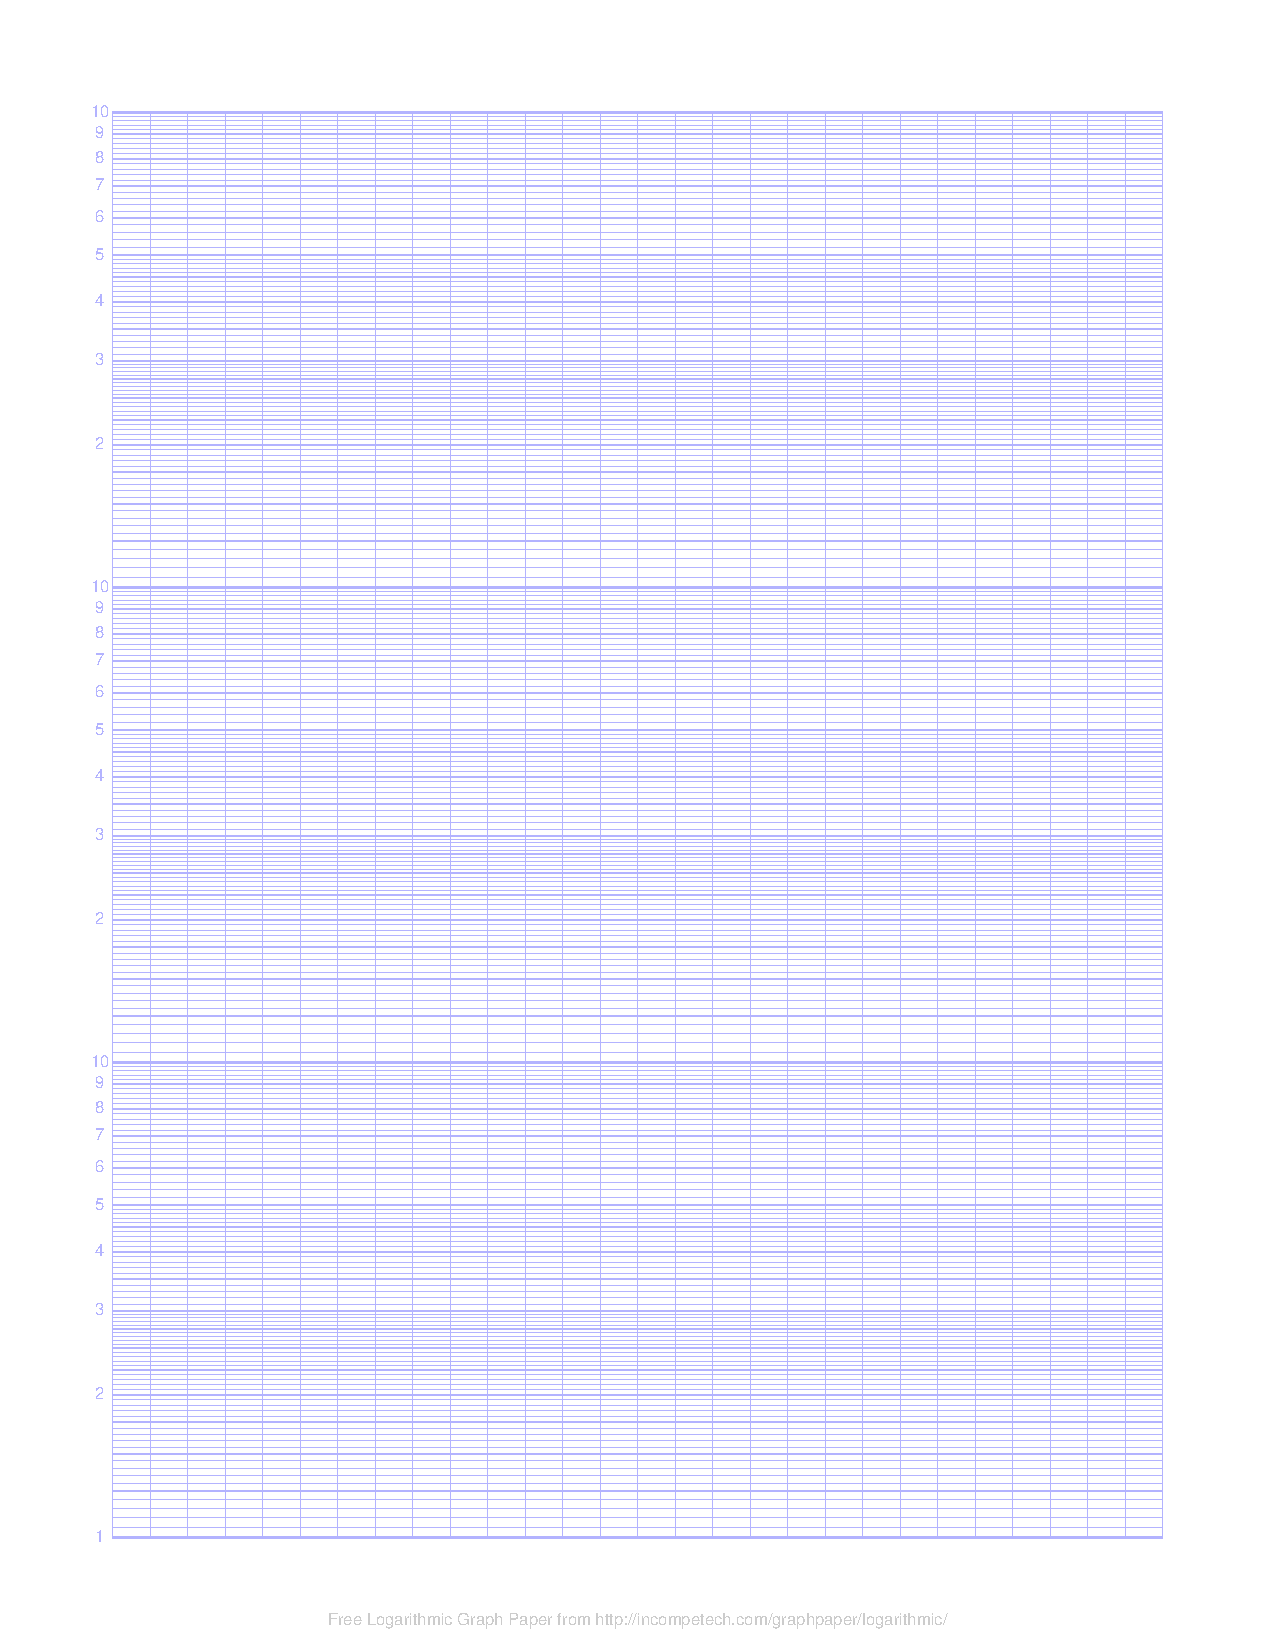
\includegraphics[width=1.3\textwidth]{semiloggraph.pdf}
\end{figure}
	





\section*{Result}
A tuned amplifier was implemented using IFT.\\
Its maximum gain= \\
Resonant frequency, $f_0$= \\
Band-width, $BW$ =\\
Q-factor=$\frac{f_0}{BW}$



\chapter[AM generation using IFT]{AM generation using IFT}

\section*{Aim}
To design and set-up  an AM generator using BJT and IFT and measure the modulation index from the observed output waveform.

\section*{Theory}
Any amplifier can be converted into a sinusoidal oscillator if Barkhausen conditions are satisfied. So tuned amplifier in chapter \ref{iftamplifier} can be converted ito a high frequency oscillator for generating carrier wave by providing a positive feedback after removing  the input and the load resistor $R_L$.

Inorder to obtain the feedback signal to the base, the terminal-1 of the IFT primary coil is used. It is $180^{\circ}$ out of phase with the signal at collector, ie. terminal-2 of IFT primary winding. The collector signal is already $180^{\circ}$ out of phase with the input signal at base of BJT. Thus the feed back signal from terminal-1 of the IFT to the base of BJT is in phase with the signal at the base. The feedback capacitor is chosen to be low to avoid additional phase shift.  

The circuit now works as an oscillator generating a signal of frequency of around 455 kHz. Its amplitude, $E_c$ can be adjusted by varying the potentiometer connected in series with the emitter resistance and frequency, $f_c$ by tuning the IFT.
\begin{equation}
e_c\ =\ E_c\ sin(2\pi f_ct)
\end{equation}
The carrier thus generated can be modulated using an audio frequency message signal by connecting it at the emitter of the transistor. It can be of frequency varying from 1kHz to 5 kHz. The amplitude can be varied in the rage of 1 V to 10 V which changes the modulation index. The modulation index can also be varied by adjusting the carrier amplitude with the potentiometer connected at the emitter.


\paragraph{}
The ratio of the maximum amplitude of the modulating signal voltage to that of the carrier voltage is termed as modulation index. This is represented as $m=\frac{E_m}{E_c}$. For both carrier and message being sinusoidal, the modulation index will be 
$m=\frac{E_{max}-E_{min}}{E_{max}+E_{min}}$
\noindent where $E_{max}$ and $E_{min}$ are respectively the maximum and minimum height of the positive side of modulated signal.
\section*{Design}
The basic biasing of the transistor is as discussed in the chapter \ref{iftamplifier}.\\
To make the circuit an oscillator, remove input signal and the load.\\
Positive feed back signal to base is taken from terminal-1 of IFT and given to base through a small capacitance of $C_1=100 pF$. \\
The emitter resistance can be raplaced with a fixed resistance of $R_E=1k\Omega$ in series with a potentiometer of $R_3=5k\Omega$.\\
The modulating signal is connected through a capacitor of $C_E=10\mu F$.
\section*{Circuit Diagram}
The circuit diagram is shown in Fig. \ref{amiftpng}
\begin{figure}
\includegraphics[width=\textwidth, height=9cm, trim=9cm 5cm 8cm 6cm,clip=true]{amift.png}
\caption{Circuit Diagram for AM generation using IFT}
\label{amiftpng}
\end{figure}
\section*{Procedure}

\begin{enumerate}
\item
Set up the circuit after verifying the condition of components.
\item
Feed AF modulating signal (say, $f_m=1kHz$ and $E_m=5mV$) using a function generator.
\item
Adjust amplitude and frequencies of the AF and carrier signals and observe amplitude modulated waveform on the CRO.
\item
Fix $f_m$ and $f_c$. Note down $E_{max}$ and $E_{min}$ of the AM signal and calculate modulation index according to the formula ,
\begin{equation}
m=\frac{E_{max}-E_{min}}{E_{max}+E_{min}}.
\end{equation}
Here $E_{max}$ is the maximum of the positive envelope of the carrier and $E_{min}$ is the minimum of the positive envelope of the carrier.
\item
Repeat for different values of $E_m$ and $E_c$. Observe the AM waveforms for different values of m.
\item
Plot the waveforms on a graph sheet.
\item

Fill in the observation column
\end{enumerate}


\section*{Observation}


\begin{figure}[h]

\includegraphics[width=\textwidth,height=15cm]{AMmodindex.png}
\caption{Effect of modulation index on AM. Sample graph}
\label{AMmodindex1}
\end{figure}
\noindent Figure. \ref{AMmodindex1}  shows the effect of modulation index on the resultant AM wave\footnote{Image source: \url{https://commons.wikimedia.org:/wiki/File:Amplitude_Modulated_Wave-hm-64.svg}}
\begin{center}

\begin{tabular}{|l|l|l|}

\hline
 & &\\
 
$E_{min}$  & $E_{max}$ & $m=\frac{E_{max}-E_{min}}{E_{max}+E_{min}}$ \\
 & & \\ \hline
 & & \\ \hline
& & \\ \hline
& & \\ \hline
\end{tabular}
\end{center}

\section*{Result}
Implemented the AM modulation circuit using BJT and IFT. Tabulated the modulation index by varying the amlitudes of message and the carrier.

\begin{figure}
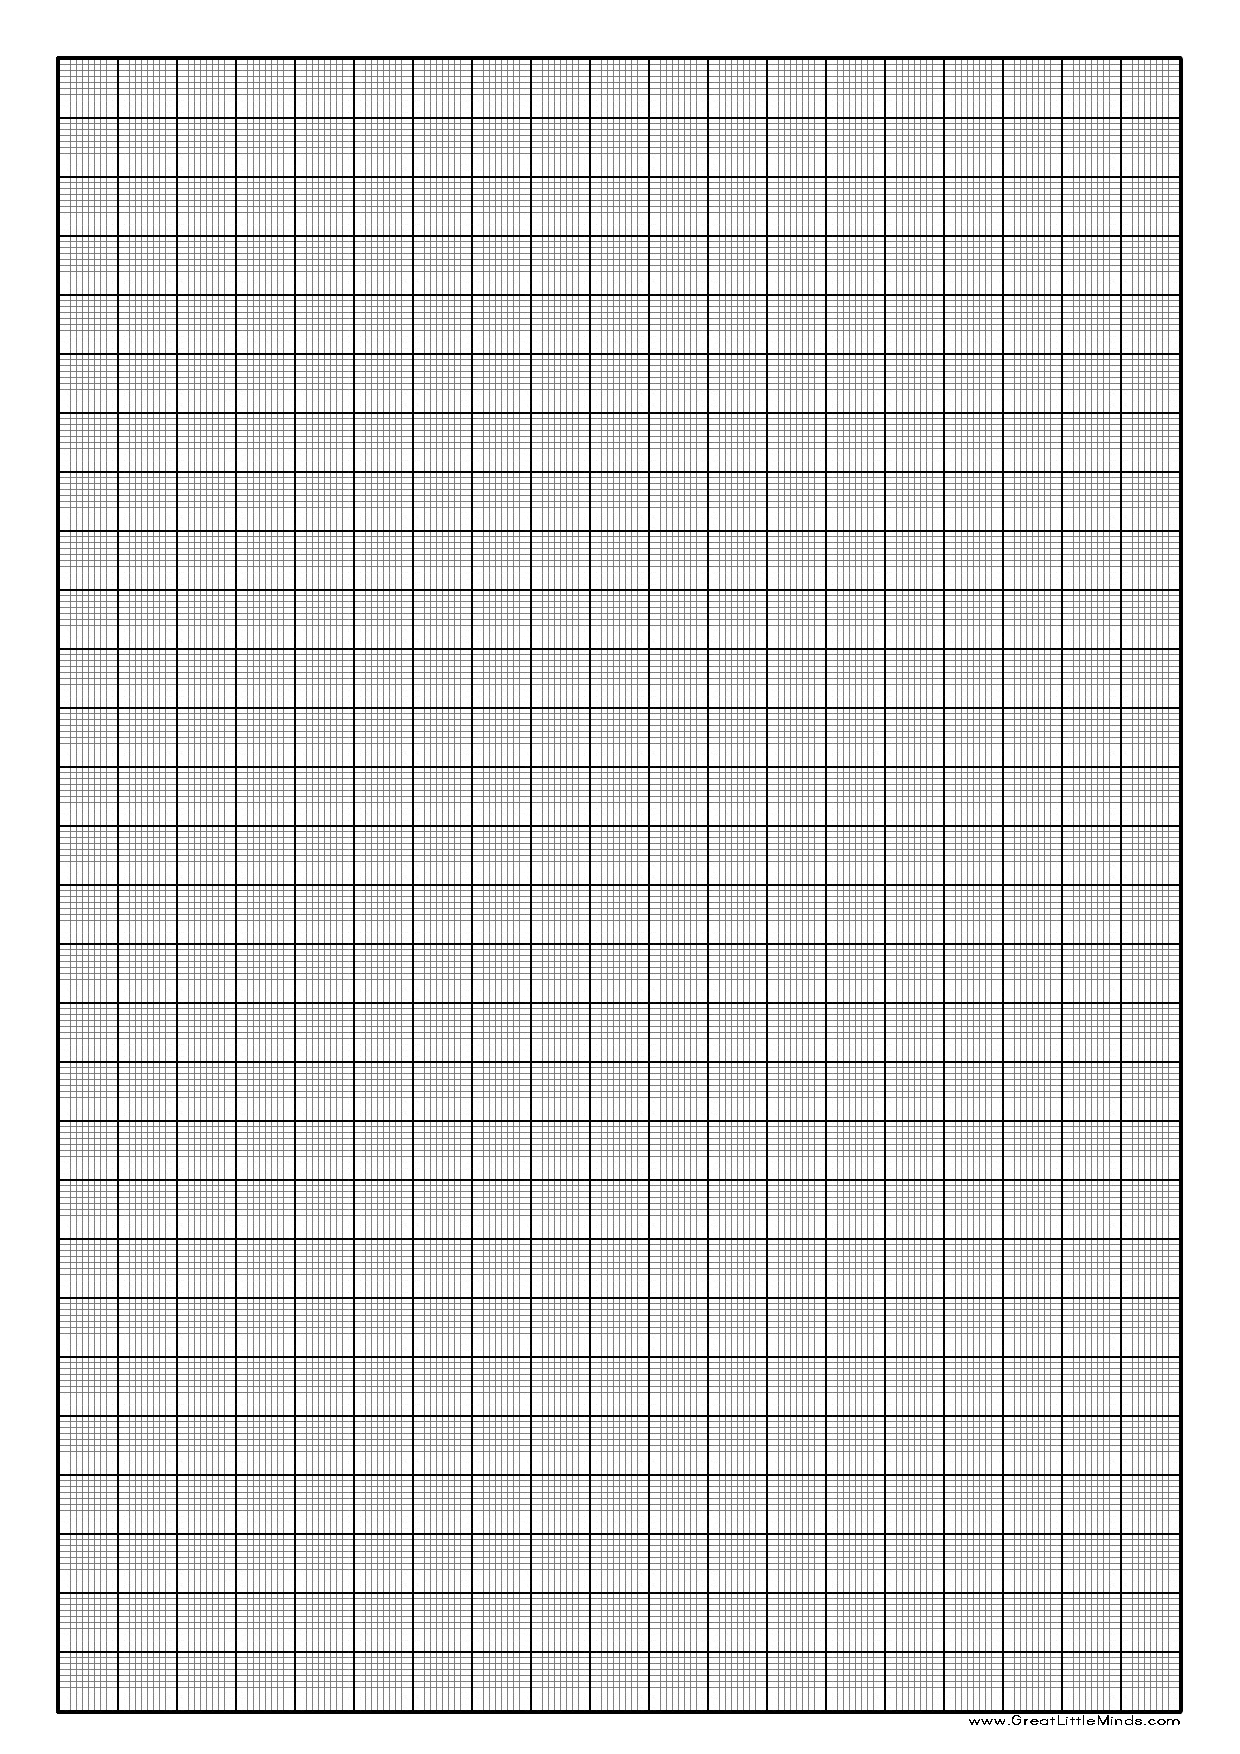
\includegraphics[width=1.1\textwidth]{graph.pdf}
\end{figure}




\chapter[AM Detection with Automatic Gain Control]{AM Detection with Automatic Gain Control}
\label{agcdetect}
\section*{Aim}
To demodulate the message content from AM signal. Also detect the automatic gain control signal from the received AM signal.
\section*{Theory}


A simple AM demodulator is a diode envelope detector. It can be implemented by a simple diode envelope detector to eliminate the negative half of the carrier envelope followed by a simple RC filter to remove the high frequency carrier. The result will be the low frequency envelope which is the demodulated message.

A point contact diode with low junction capacitance is used in the circuit as it is has to rectify high frequency carrier. It offers low impedence at high frequency. The RC elements connected after the diode acts as a filter. It acts as a lowpass filter which eliminates high frequency carrier at the same time it retains the low frequency message signal. 

Thus the output of the filter contains the low fequency modulating signal with a dc offset. The dc offset voltage is proportional to the strength of the modulated signal received by the receiver in a transmission reception system, which inturn is proportional to the strength(amplitude) of the carrier. This dc value may be used for automatic gain control(AGC) of intermediate frequency(IF) amplifier stages. The Automatic gain control compensates for minor variations in the received RF signal level. The AGC circuit automatically increases the receiver gain for weak RF input levels and automatically decreases the receiver gain when strong RF signal is received\footnote{For detailed explanation, refer to Chapter 5 of \cite{Tomasi}}.
\paragraph{Simple AGC:} It is implemented in the form of a circuit which extracts the dc offset voltage which is present along with the demodulated message. This volatge is fed as degenerative or negtive feedback to the control the gain of superheterodyne receivers. 
\paragraph{Delayed AGC:}In simple AGC circuits even if the signal level received is low, the AGC circuit operates and the overall gain of the receiver gets reduced. To avoid this situation, a delayed AGC circuit is used. In this case AGC bias voltage is not applied to amplifiers, until signal strength has reached a predetermined level after which AGC bias is applied like simple AGC.

\section*{Design}

After the positive envelope detector, a properly designed low pass filter is added to filter out the high frequency carrier and to retain the low frequency modulating signal. This signal contains a dc level also which can be used for automatic Gain Control (AGC) for the IF amplifier stages of a superhetrodyne receiver.\\

\noindent Let the carrier frequency be $f_c=455\ kHz$ and maximum modulating signal frequency be $f_m=10\ kHz$

\noindent Inorder to design a lowpass filter with upper cutoff frequency 10 kHz,
\begin{equation}
f_H=\frac{1}{2\pi R_dC_d}
\end{equation}
\begin{equation}
10\ kHz=\frac{1}{2\pi R_dC_d}
\end{equation}
\noindent Select $C_d=\ 0.001 \mu F$. Then $R_d=\ 16.1k\Omega$.
Choose $R_d=\ 15k\Omega \ or\ 22k\Omega$ standard resistor values.\\

\noindent Make a $\pi$ filter (for better performance) using these $R_d$ and $C_d$ values. This completes the envelope detector part.
\paragraph{AGC Circuit:} The AGC lowpass filter $R_a$ and $C_a$ is seected in such a way as to eliminate full ac from the output and get a pure dc AGC voltage. 
Hence assuming a cutoff frequency of 10 Hz to eliminte the fluctuations,
\begin{equation}
10 Hz= \frac{1}{2\pi R_aC_a}
\end{equation}
\noindent Assuming $C_a=1 \mu F$, we get $R_a=22 k \Omega$

The actual modulating signal can be obtained by  filtering out the dc components using a high value caacitance like  $10\mu F$.

%\paragraph{Delayed AGC Circuit:}
%Here the simple AGC circuit is applied to a difference amplifier.  Delayed AGC output will be produced only when input voltage $V_i$ exceeds the threshold voltage which can be set to the desired value by adjusting the dc level of the potentiometer.
%
%LM 741 opamp is chosen as the amplifying element. It is configured in difference amplifier mode. The Simple AGC volatge derived from previous 
%circuit is used as the input to the inverting terminal of the  difference amplifier throgh the input resistance $R_i$. The threshold voltage is set at the non-inverting terminal. The voltage at non-inverting terminal can be varied in between +12V and 0V.
%
%The gain of the difference volatage is determined by the values of feedback resistance $R_f$, input resistance $R_i$ and the position of variabale terminal of the potentiometer. The opamap is biased using +12V and -12 V respectively. 
%The values of ristances are chosen as:

%\begin{equation}
%R_i\ =\ R_f\ =R_{pot}\ =100 k \Omega
%\end{equation}
\section*{Circuit Diagram}
The detector circuit with simple AGC is shown in Figure. \ref{detectagcckt}.%and with delayed AGC is shown in Fig. \ref{delayedagcckt}.
\begin{figure}

\includegraphics[height=8cm,width=15cm, trim=0cm 2cm 0cm 3cm,clip=true]{amdetectagc.png}
\caption{Detector circuit with Simple AGC}
\label{detectagcckt}
\end{figure}

%\begin{figure}
%
%\centering \includegraphics[height=8cm,width=12cm, trim=0cm 0cm 0cm 3cm,clip=true]{delayedagc.png}
%\caption{Detector circuit for delayed AGC}
%\label{delayedagcckt}
%\end{figure}
\section*{Procedure}
\begin{enumerate}
\item
Connect the diode to the output of AM signal(See Figure. \ref{amenv}) as in the circuit diagram Fig. \ref{detectagcckt}.
\item
Connect load resistance $R_L$ and observe the outputwaveform on a CRO and plot it.
\item
Connect the $\pi$ filter circuit of $R_d$ and $C_d$ and observe the output waveform on a CRO and plot it.
\item
Obtain the demodulated output without dc offset by connecting capacitor $C_3$. Observe it on a CRO and plot it.
\item
Connect the lowpass filter using $C_a$ and $R_a$ for obtaining AGC voltage level. Observe it on a CRO and plot it.
\item Vary the modulation index by changing carrier or modulating signal levels. Plot the simple AGC charateristics with modulation index on x-axis and AGC voltage level on y-axis.
\item
Eliminte the dc offset and observe the modulating signal from the $10\mu F$ capacitor as shown in the circuit diagram.
%\item
%Feed the AGC voltage to the delayed AGC	circuit of Fig. \ref{delayedagcckt}.
%\item
%Set the threshold to a fixed value, say $V_{threshold}=).5 V$. Keep the carier amplitude to the lowest, so that modulation index is 1.
%\item
%Slightly go on increasing the carrier amplitude. Note that for small values of carrier amplitude, delayed AGC voltage is positive. When it is above a certain limit the delayed AGC value becomes negative.
\end{enumerate}
\section*{Observation}
The following are the observed results of the experiment. See Figure. \ref{aminter} and Figure. \ref{demodagcwaves} for the sample waveforms of intermediate and final stages.
\begin{figure}
\includegraphics[height=8cm, width=12cm]{am.png}
\caption{AM with message envelope}
\label{amenv}
\end{figure}
\begin{figure}
\includegraphics[height=8cm, width=12cm]{demodfig.png}
\caption{Intermediate stage of demodulation}
\label{aminter}

\end{figure}
\begin{figure}
\includegraphics[height=8cm, width=\textwidth]{demodagc2.png}
\caption{Output waveforms from demodulation circuit}
\label{demodagcwaves}
\end{figure}

\begin{figure}
	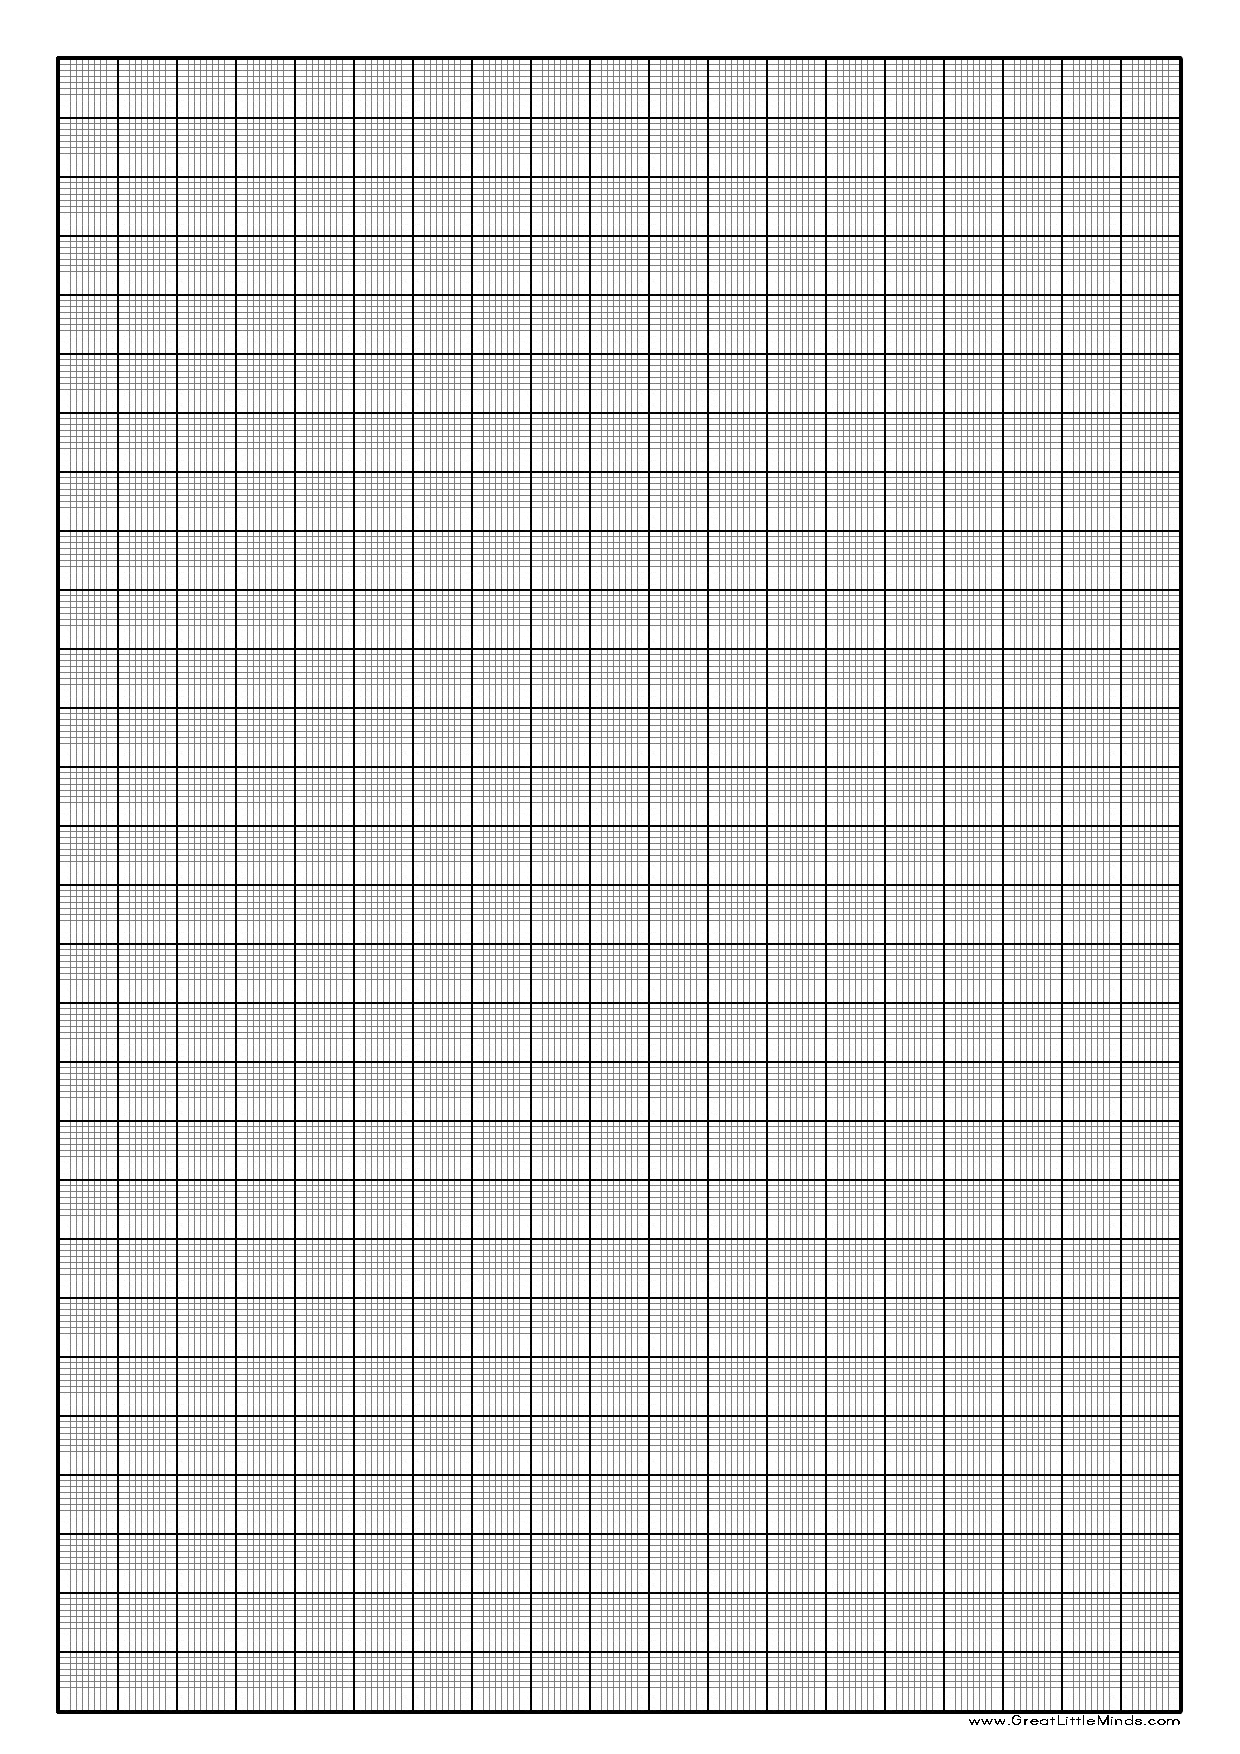
\includegraphics[width=1.1\textwidth]{graph.pdf}
\end{figure}

\begin{figure}
	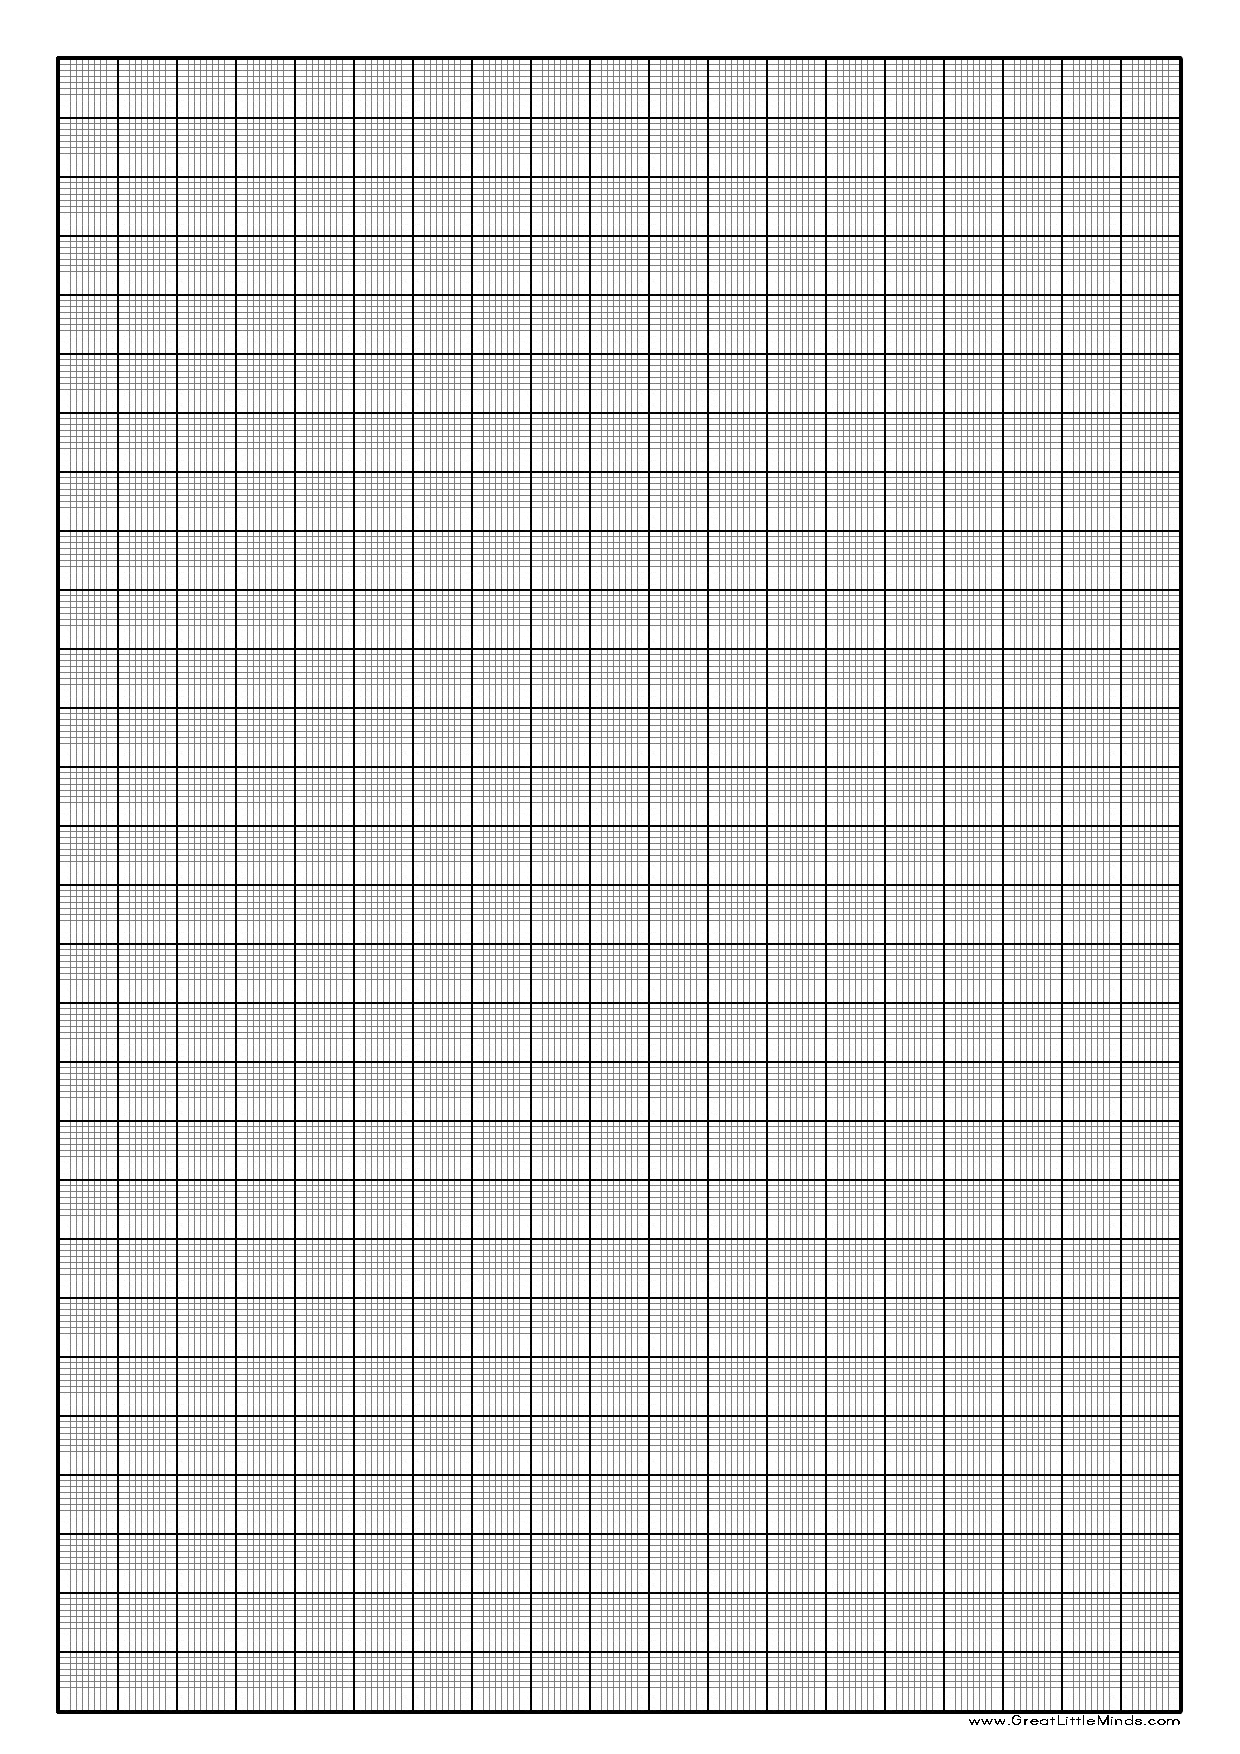
\includegraphics[width=1.1\textwidth]{graph.pdf}
\end{figure}


\section*{Result}

Demodulation circuit was designed and implemented with simple AGC. Details of obeserved outputs are indicated and plotted on graph.

\input{chapters/BalancedModulatorforDSBSC.tex}

\chapter[AM generation and Demodulation using AD 633]{AM generation and Demodulation using AD 633}
\section*{Aim}
To design and implement AM generation and demodulation using multiplier IC AD633.
\section*{Theory}
DSB-SC using AD633 has already been discussed in chapter \ref{chapdsbsc}. DSB-SC is same as AM devoid of the carrier. Inorder to obtain the complete AM waveform which is \emph{double side band with carrier}, add the carrier signal to the DSB-SC signal. This can be done using the 633 multiplier IC. For more details on IC, refer \ref{AD633}.
\begin{equation}
W= \frac{X.Y}{10}+Z
\end{equation}
\begin{equation}
W= \frac{Emsin(2\pi f_mt).Ecsin(2\pi f_ct)}{10}+E_c sin(2\pi f_ct)
\end{equation}
\begin{equation}
W= \frac{E_mE_c [cos (2\pi (f_c\ -\ f_m)t)]}{20}- \frac{E_mE_c[cos (2\pi (f_c\ +\ f_m)t)]}{20}+E_c sin(2\pi f_ct)
\end{equation}

\paragraph{}
	The resultant AM can be demodulated in two ways,
 \begin{enumerate}

\item
Using Diode envelope detector.
\item
Using another AD633 in cascade with AM generating circuit for multiplying the AM with the carrier.
\end{enumerate}

Multiplying the AM with the carrier once again will result in the following output.
\begin{equation}
\begin{split}
W=\frac{1}{10} &[ \frac{E_mE_c [cos (2\pi (f_c\ -\ f_m)t)]}{20}- \frac{E_mE_c[cos (2\pi (f_c\ +\ f_m)t)]}{20}\\
&\quad +E_c sin(2\pi f_ct)].E_c sin(2\pi f_ct)
\end{split}
\end{equation}

\begin{equation}
\begin{split}
W=& \frac{{E_c}^2}{20}+\frac{E_m.{E_c}^2}{200}sin(2\pi f_mt) \\
&\quad -\frac{{E_c}^2}{20}cos(2\pi(2f_m)t) \\
&\quad +\frac{E_m.{E_c}^2}{400}sin(2\pi (2f_c-f_m)t)  -  \frac{E_m.{E_c}^2}{400}sin(2\pi (2f_c+f_m)t)
\end{split}
\end{equation}

Thus the signal consists of various frequencies of which, the smallest is the message frequency. It can be extracted by filtering using a low pass filter. Since the amplitude of the message frequency is very small, It may be amplified using a simple non-inverting amplifier using an opamp.

\section*{Design}
Provide the supply voltage of +15 V to pin 8 of the IC and -15 V to pin 5 of the IC.\\

\noindent To the \textbf{Y} and \textbf{Z} inputs of the IC, feed the carrier sinusoid of amplitude $E_c=2.5\ V$ and frequency $f_c= 100\ kHz$.\\
To the \textbf{X} input of the IC, feed the message sinusoid of amplitude $E_m=2.5\ V$ and frequency $f_m= 1\ kHz$.\\

\noindent The output AM signal will have a waveform as given by,

\begin{equation}
W=\frac{X.Y}{10}+Z
\end{equation}
\begin{equation}
W=\frac{e_m.e_c}{10}+e_c
\end{equation}
\begin{equation}
W=\frac{6.25}{20}[cos 2\pi 99kt-cos 2\pi 101kt]+2.5 sin(2\pi100kt)
\end{equation}

\noindent Thus it contains two sidebands and the carrier, ie \emph{Double sideband - Full Carrier AM}.
\paragraph{Demodulation:}
Detection may be done using a diode envelope detector as already discussed in chapter \ref{agcdetect}.

An alternate method of demodulation is by multiplying the AM signal once again with the carrier. This can be implemented by connecting another AD633 IC in cascade with the first one.

\noindent The multiplication will result in the following output, as per the theory already explained.

\begin{equation}
\begin{split}
W=& \frac{6.25}{20} +\frac{15.625}{200}sin(2\pi 1kt)\\
&\quad  -\frac{6.25}{20}cos(2\pi 2kt) +\frac{15.625}{400}sin(2\pi199kt) -\frac{15.625}{400}sin(2\pi 201kt)
\end{split}
\end{equation}

\noindent This waveform is shown in Figure \ref{AM633plot2}, which is the stage -1 in demodulation. The next step is to obtain the message signal. This is done by lowpass filtering the above signal at a cut-off frequency of 1.5 kHz.

To design an RC lowpass filter of cut-off frequency 1.5 kHz,

\begin{equation}
f_c=\frac{1}{2\pi R_1C_1}=1.5kHz
\end{equation}
Choose $C_1=0.01\  \mu F$
$\therefore  R_1 =10 \ k \Omega$

A non-inverting amplifier may be used to amplify this signal. Using a feedback resistor of $R_f= 100 \ k \Omega$ and an input resistance of $R_i=10\ k\Omega$ will result in a gain of $A_v=1+\frac{R_f}{R_i}=11$.
\section*{Circuit Diagram}
The circuit diagram for generating AM(DSB-FC) and demodulating it using AD633 multiplier IC as shown in Figure. \ref{633amckt}. 

\begin{sidewaysfigure}[ht]
    \includegraphics[scale=0.8, trim=0cm 4cm 0cm 4cm,clip=true]{633amckt.png}
    \caption{Circuit for AM generation and detection using AD633 multiplier IC}
    \label{633amckt}
\end{sidewaysfigure}


\section*{Procedure}
\begin{itemize}
\item
Make connections as shown in the circuit diagram, figure \ref{633amckt}.
\item
Feed the message and carrier signals.
\item
Connect the pin number 7 of the first IC to a CRO and observe the resultant waveform which is AM(DSB-FC).
\item
Connect the pin number 7 of the second IC to a CRO and observe the resultant waveform which is the product of DSB-FC and the carrier.(Named demodulation stage-1 signal)
\item
Observe the output from the filter, amplified by the opamp amplifier, which extracts the envelope of the signal-\emph{The 1kHz message signal}.
\item
Plot the signals observed on a graph sheet.
\end{itemize}
\section*{Observation}
The samples of input and output signals as observed on a CRO are shown in Figure \ref{AM633plot1}and \ref{AM633plot2}.

The experimentals observations are noted and plotted on graph.
\begin{figure}[ht]
\includegraphics[width=\textwidth]{am6331.png}
\caption{Message and carrier signals}
\label{AM633plot1}
\end{figure}

\begin{figure}[ht]
\includegraphics[width=\textwidth]{am6332.png}
\caption{AM(DSB-FC) and Demodulation stage-1 signals}
\label{AM633plot2}
\end{figure}

\begin{figure}
	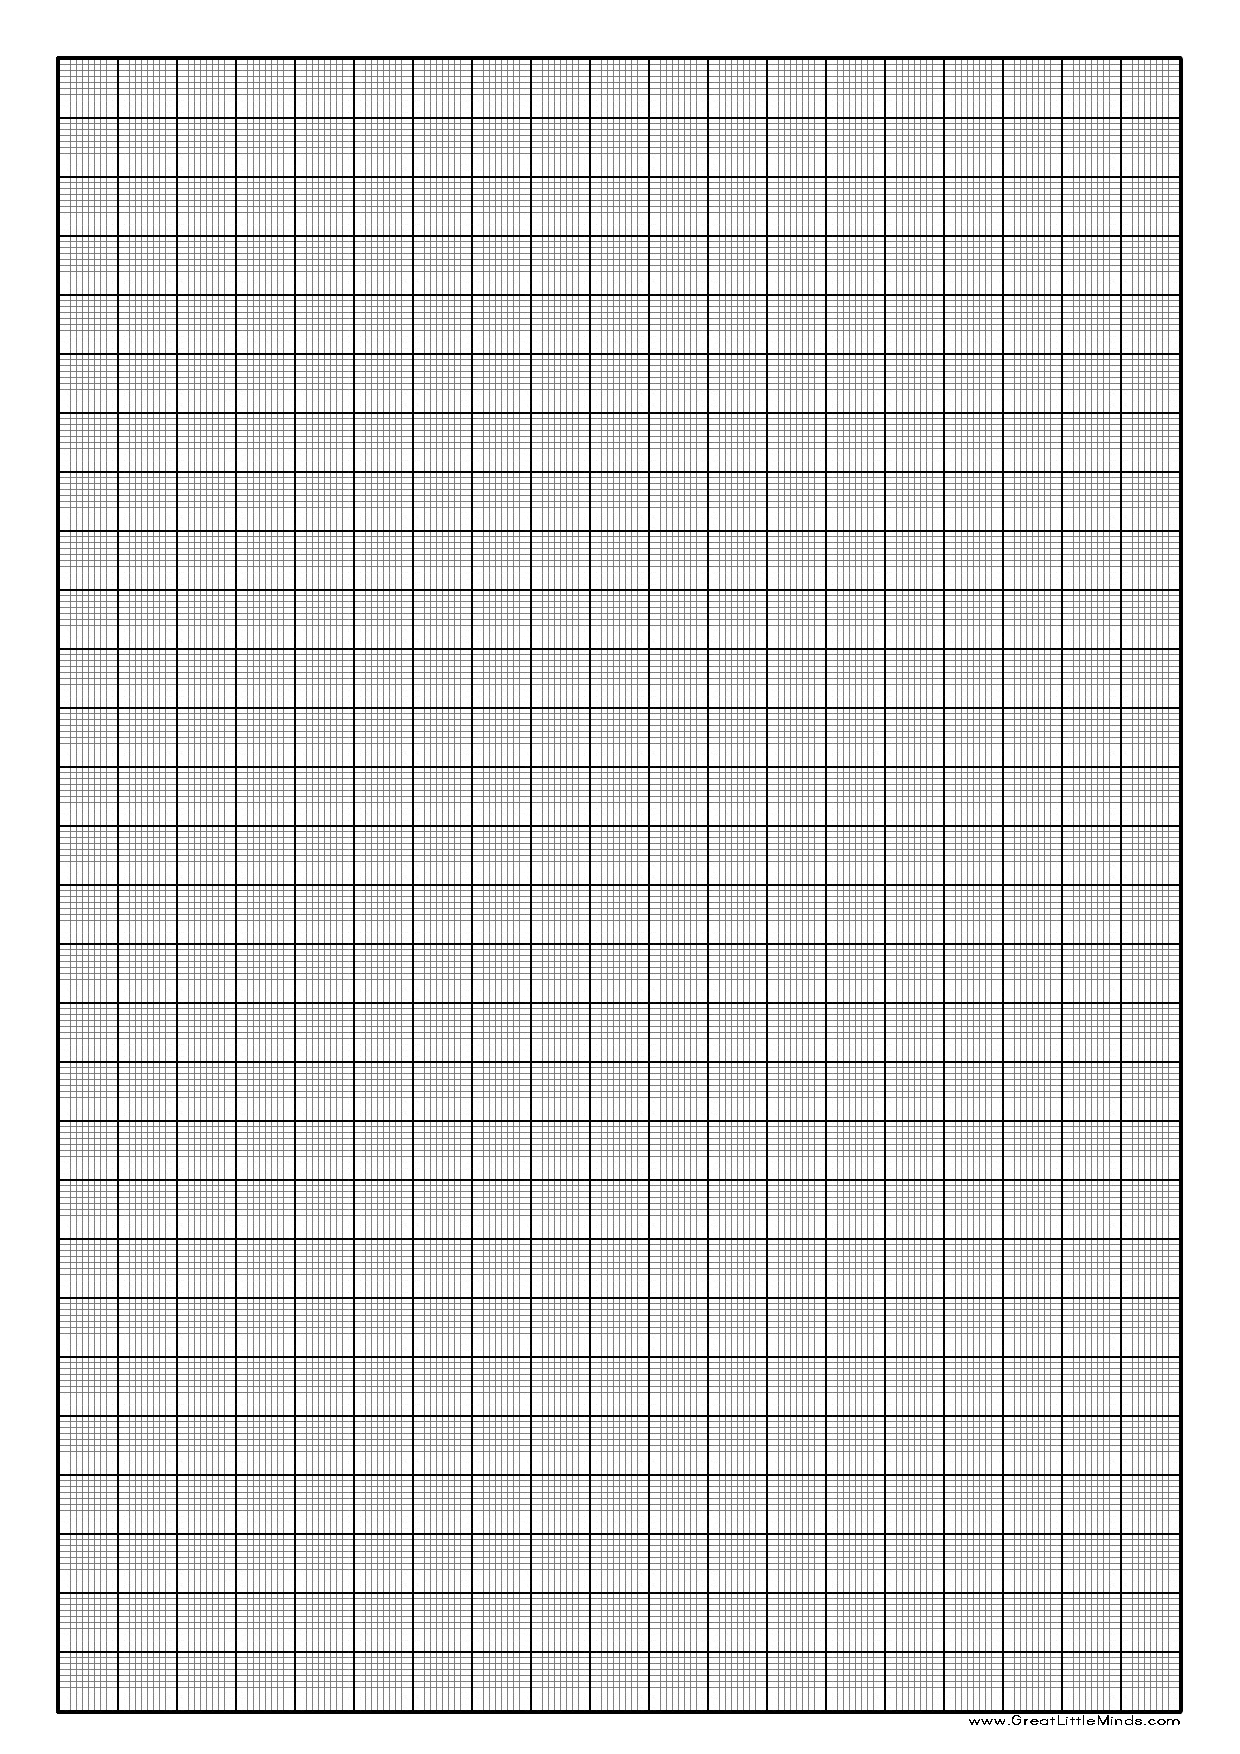
\includegraphics[width=1.1\textwidth]{graph.pdf}
\end{figure}

\begin{figure}
	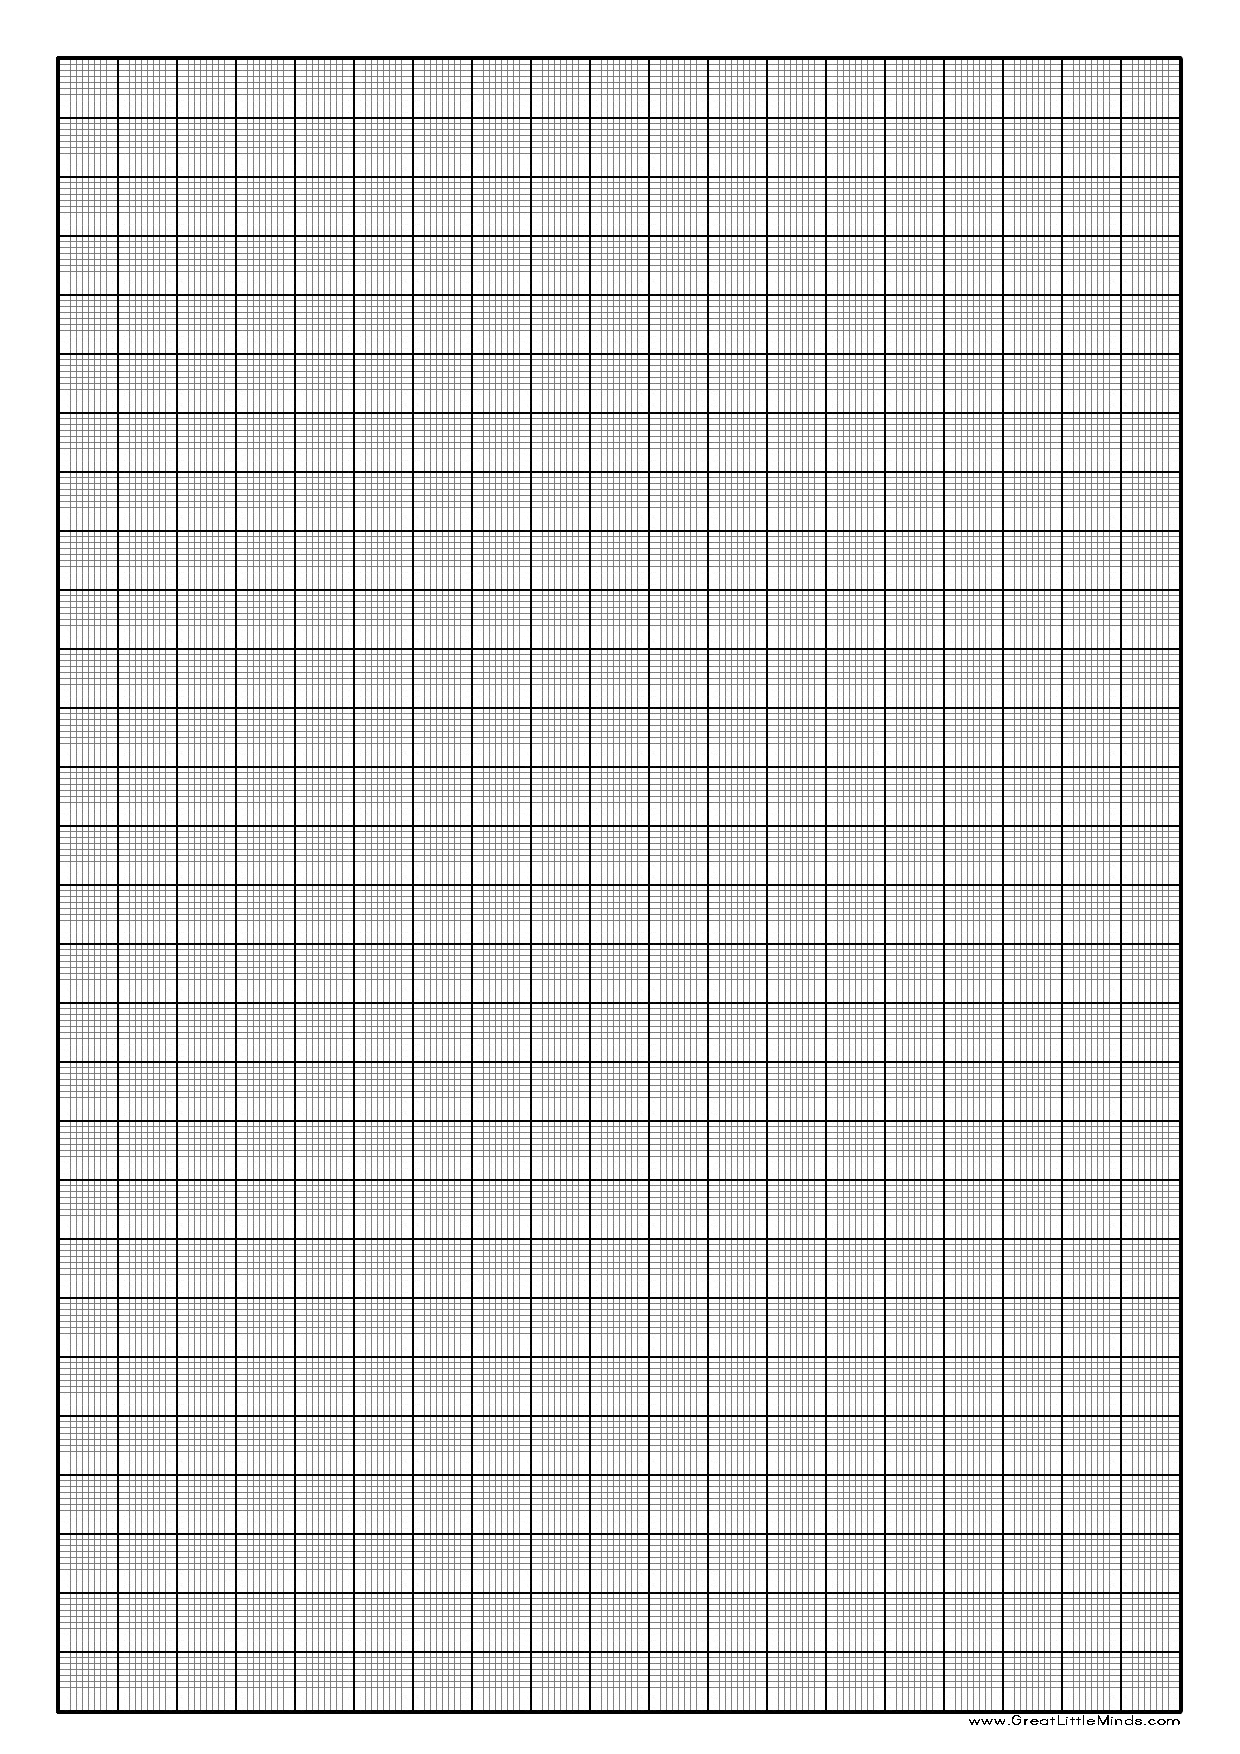
\includegraphics[width=1.1\textwidth]{graph.pdf}
\end{figure}



\section*{Result}
Implented the AM generation and demodulation circuit using multiplier IC and opamps.
The resultant waveforms were plotted.
\chapter[FM using 555]{FM using 555}

\section*{Aim}
To design and set up a frequency modulating circuit using 555.

\section*{Theory}
Frequency modulation is an analog modulation technique in which the frequency of the carrier is varied in accordance with the message signal amplitude.
Modulation index for FM is 
\begin{equation}
m= \frac{\delta f}{f_m}=\frac{frequency \ deviation}{modulating \ signal\  frequency}
\end{equation}

555 is an IC which can be used to to set up an astable multivibrator of 50\% duty cyle whose frequency is determined by externally connected RC load. \emph{(See Appendix \ref{555}})

\noindent The standard design equation for an astable mutivibrator using 555 timer IC is defined by the following equation for its time period.
\begin{equation}
T=1.38 \ RC
\end{equation}

\noindent Thus its frequency of oscillation is 
\begin{equation}
f_0 = \frac{0.72}{RC}
\end{equation}
This frequency of oscillation remains constant as long as the pin-5 is supplied with a constant voltage. If the voltage at pin-5 is varying the frequency of oscillation of the astable multivibrator also changes along with it.

Thus astable multivibrator using 555 can be used as a carrier pulse generator. The frequency of the carrier can be varied by feeding the pin-5 with message signal.
\section*{Design}
\noindent Let the carrier frequency be given by $f_c= 10 kHz$
\begin{equation}
f_c=\frac{0.72}{RC}
\end{equation}
\noindent Let $C=0.01 \mu F$
\begin{equation}
\therefore
R=\frac{0.72}{(10) (10^3)(0.01 X 10^-6)}= \ 6.8 k\Omega
\end{equation}

The amplitude of the modulationg signal should be limited by $\frac{2}{3}V_{cc}$. This is needed to avoid over modulation. The message signal should have a frequency less than 1 kHz.

The dc supply voltage of the IC, 
\begin{equation}
V_{cc}=12 V
\end{equation}
\begin{equation}
\therefore V_{m_{pp}}=\frac{2}{3}X12 V=8V
\end{equation}
\section*{Circuit Diagram}
The circuit to implement frequency modulation using 555 is shown in Figure \ref{fm555ckt}.

\begin{figure}
\includegraphics[height=7cm,width=\textwidth,trim=2cm 3cm 2cm 2cm,clip=true]{fm555.png}
\caption{Circuit to implement frequency modulation using 555}
\label{fm555ckt}
\end{figure}

\section*{Procedure}

\begin{itemize}
\item
Make connections as per the circuit diagram.

\item

Feed the message signal of peak-to-peak amplitude of 5V and frequency 1kHz.
\item Observe the FM output at pin number-3.

\item
Plot the observations on a graph sheet.
\end{itemize}


\section*{Observations}
Observe the input and output waveforms on a CRO and plot the same on a graph sheet. See Figure \ref{fmwaves}.


\begin{figure}
\begin{center}
\includegraphics[height=7cm,width=10cm]{fm.png}
\caption{Message, Carrier and frequency modulated waveforms}
\label{fmwaves}
\end{center}


\end{figure}


\begin{figure}
	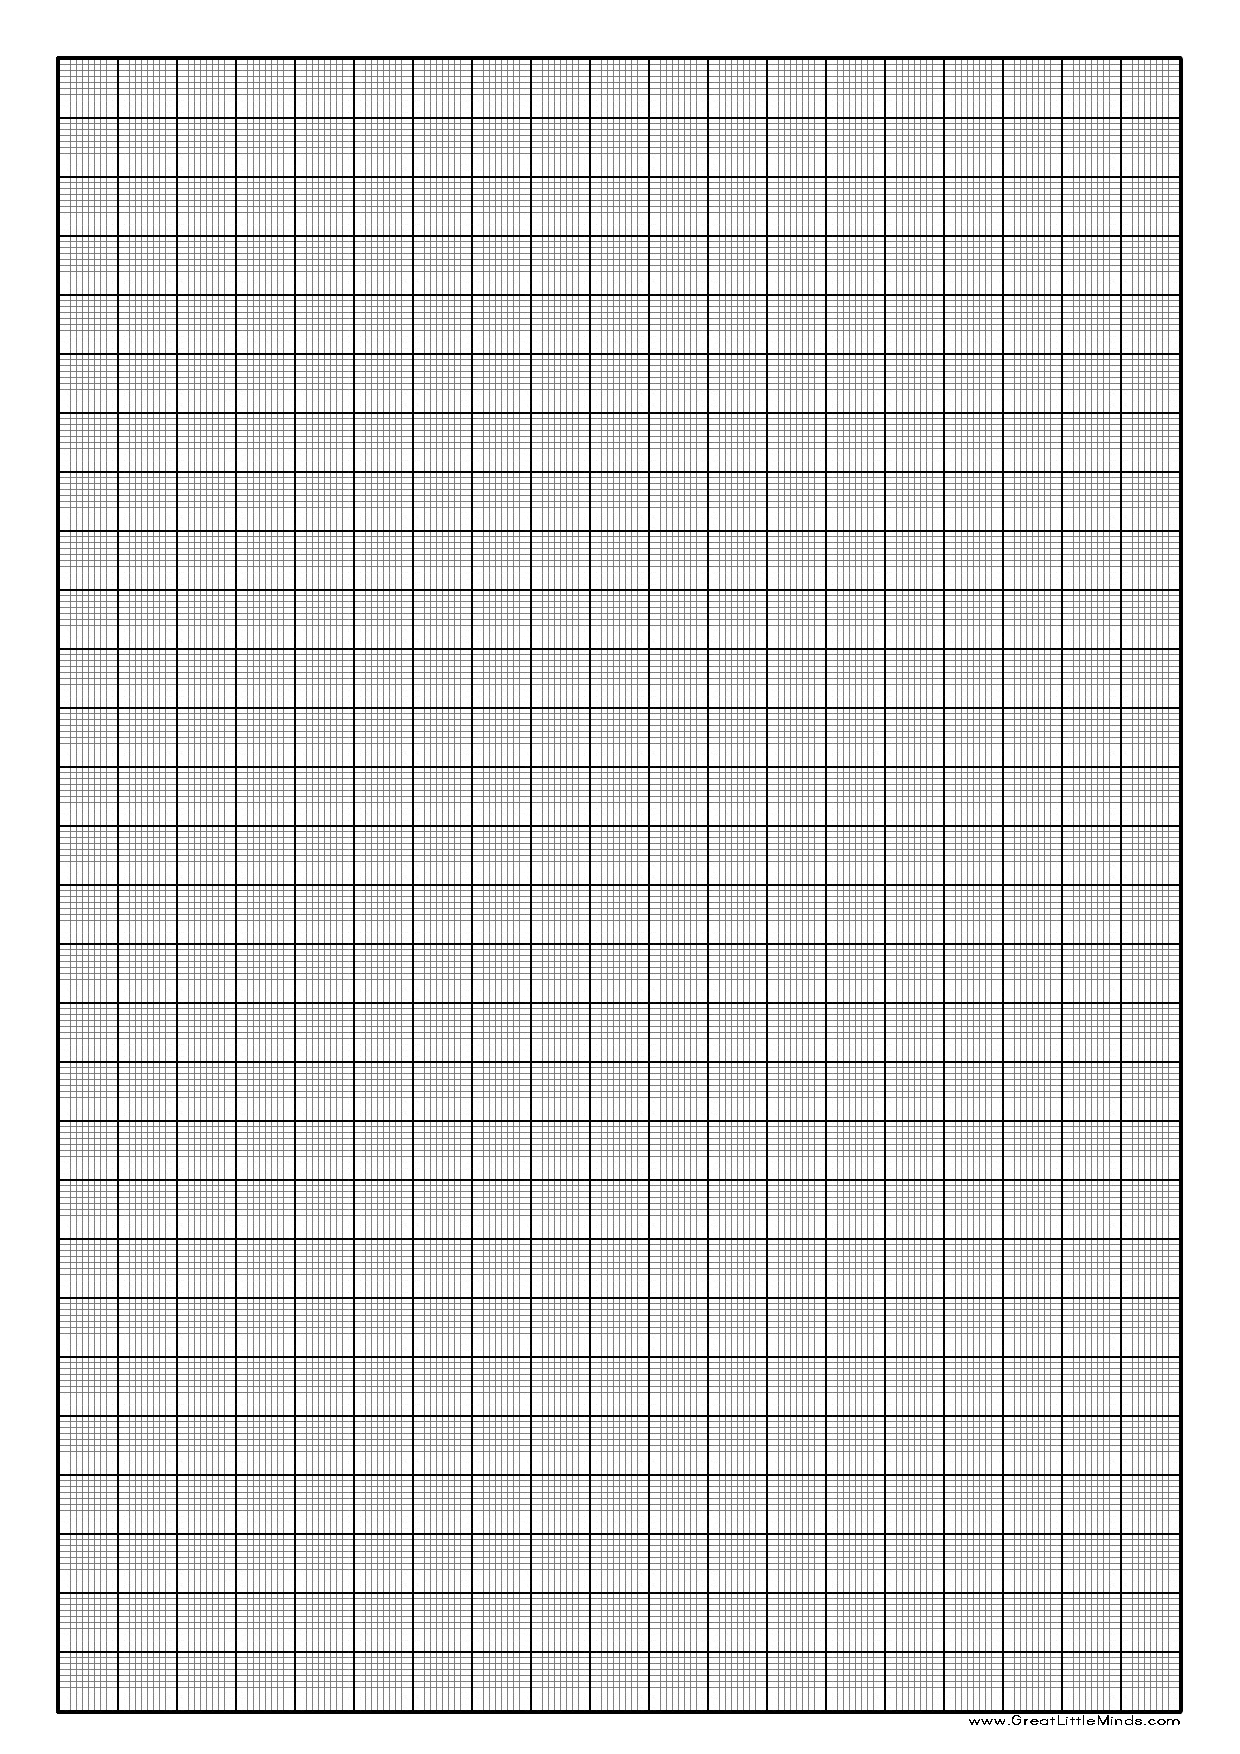
\includegraphics[width=1.1\textwidth]{graph.pdf}
\end{figure}



\section*{Result}
Implemented frequency modulation of pulse carrier by sinusoidal messaage using 555 timer IC.





\input{chapters/pll.tex}
\input{chapters/fmpll.tex}
\input{chapters/mixerbjt.tex}

\chapter[PAM Generation and Demodulation]{PAM Generation and Demodulation}

\section*{Aim}
To set-up and implement circuits to carry out pulse amplitude modulation. To design demodulationg circuits to detect the message from pulse amplitude modulated wave.
\section*{Theory}
Pulse amplitude modulation is a kind of digital modulation technique in which analog message signal is sampled at constant frequency - \emph{carrier frequency}. A pulse of specified duration is used to sample the message signal. When the pulse is on, the message is sampled and when it is off no message is sampled. This is a basic step in the digitization of analog message signals. The circuits to be implemented in this experiment does a kind of natural sampling.\footnote{For more on natural sampling, refer Digital Transmission \cite{Tomasi}}.

Waveforms showing pulse carriers whose amplitude is modulated buy message is shown in Figure \ref{PAMmod1} and \ref{PAMmod2
}. A simple way to implement this is to allow the message to be fed as the input to a switch and the switch ON/OFF time is controlled by the pulses at sampling frequency.

The demodulation of PAM waveform can be implemented by using a lowpass filter which passes message signal frequenies but blocks the carrier signal.
\begin{figure}[h]
\includegraphics[width=\textwidth]{pam1.png}
\caption{PAM modulation using transistor}
\label{PAMmod1}
\end{figure}

\begin{figure}[h]
\includegraphics[width=\textwidth]{pam2.png}
\caption{PAM modulation using switching IC}
\label{PAMmod2}
\end{figure}
\section*{Design}
\subsection*{PAM using transistor as a switch}
One technique to implement PAM is to use transistr in switching mode. The flow of current from collector to emitter in a bipolar junction transistor is controlled by the voltage at its base. 


\noindent Choose the transistor BC107. For more details on BC107 see \ref{BC107}.
\noindent Apply the sinusoidal message signal of frequency $f_m < \ 1 \ kHz$ and amplitude $E_m<\ 10\ V_{pp}$ at the collector.
\noindent Apply a carrier at the transistor base through a resistor $10 k\Omega$. The carrier pulse amplitude is set as $E_c =10 \ V_{pp}$ and frequency $f_c=\ 10 kHz$.

\subsection*{PAM using CMOS switching IC CD4016}
CD 4016 is a quad bilateral CMOS switching IC. See \ref{4016} for more deatails. The message signal is fed to any of the input terminals of the switch and the modulating pulse carrier is fed as the control signal for the switch. The PAM output will be available at the output terminal of the switch which is fed to the CRO across a load resistor of $10\ k\Omega$. Keep the message signal frequency to be $f_m=500 \ Hz$ and the switching pulse of 10 kHz which is the carrier is to be fed  from the TTL output from a function generator.

\subsection*{Demodulation}
Demodulation is done using a  $\pi$ RC filter.
\noindent Design the filter as per the equation for upper cut-off frequency of a low pass filter,
\begin{equation}
f_H=\frac{1}{2\pi R_dC_d}
\end{equation}
\begin{equation}
1.5\ kHz=\frac{1}{2\pi R_dC_d}
\end{equation}
\noindent Select $C_d=\ 0.01 \mu F$. Then $R_d=\ 10k\Omega$.
Choose $R_d=\ 10k\Omega$ standard resistor value.\\

\section*{Circuit Diagram}
\subsection*{Using transistor as a switch}

The PAM generation using transistor as a switch and demodulation circuit is shown in Figure. \ref{pamckt}.

\begin{figure}
\includegraphics[height= 6cm, width=\textwidth, trim=5cm 3cm 4cm 4cm,clip=true]{pamckt1.png}
\caption{PAM generation and demodulation circuuit}
\label{pamckt}
\end{figure}



\subsection*{Using CMOS switching IC CD4016}
The PAM generation using CD4016 is shown in Figure. \ref{pamckt2}. Demodulation can be done in the same way as shown in \ref{pamckt}.

\begin{figure}
\includegraphics[width=\textwidth, height=7cm, trim=3cm 4cm 6.5cm 4cm,clip=true]{pamic.png}
\caption{PAM generation using CD4016}
\label{pamckt2}
\end{figure}

%\section*{Components and Equipments Required}
%CRO (1), \\Signal generator(2),
%\\Resistors: $15\ k\Omega$(2), $10\ k\Omega$(1)
%\\Capacitors: $0.01\  \mu F$(2)
\section*{Procedure}
\begin{itemize}
\item
Connect the PAM generating circuit as shown in the circuit diagram, Figure \ref{pamckt}.
\item
Feed the modulating message signal and the carrier pulses from the function generator.
\item
Observe the output on a CRO and plot the graphs of the input and output waveforms.
\item
Make the demodulating circuit as shown in the circuit diagram, Figure \ref{pamckt}.
\item
Repeat the PAM experiment using CD4016 IC.
\item
Make connections as shown in the circuit diagram Figure. \ref{pamckt2}. If IC is used for modulation make sure it is biased with $V_{DD}=5V$ and is properly grounded.
\item
Observe the input and output waveforms from PAM generaton and demodulation circuits using CD4016 IC.

\end{itemize}
\section*{Observation}
Plot the graphs of input and output waveforms as observed on a CRO.

\begin{figure}
	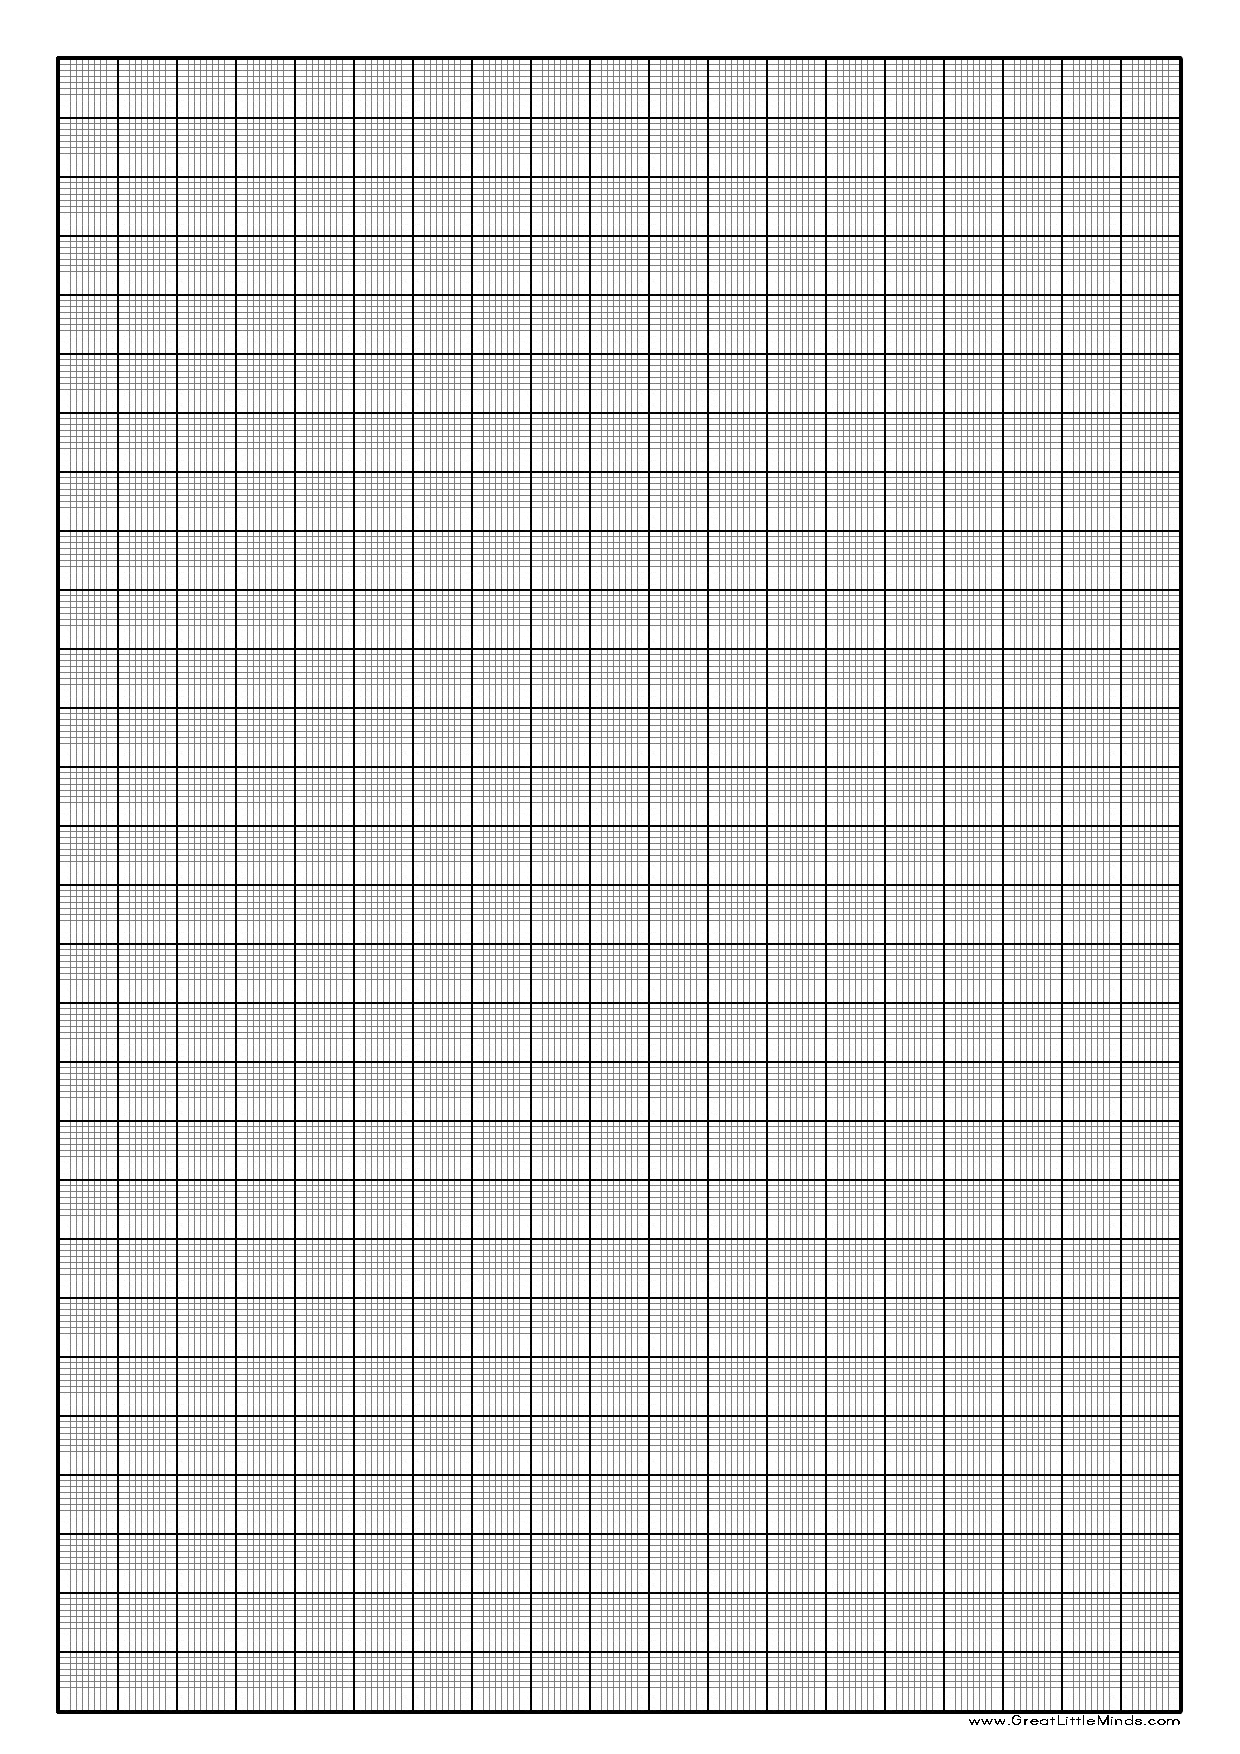
\includegraphics[width=1.1\textwidth]{graph.pdf}
\end{figure}
\section*{Result}

Implemented the PAM generation and demodulation circuits using BJT as well as switching IC.
\input{chapters/pwm.tex}
\input{chapters/ppm.tex}
\chapter[BASK Generation and Demodulation]{BASK Generation and Demodulation}

\section*{Aim}
To set-up and implement circuits to carry out Binary Amplitude Shift Keying (BASK). To design demodulationg circuits to detect the message from BASK modulated wave.
\section*{Theory}

Binary Amplitude Shift Keying or ON-OFF Keying is the simplest digital modulation technique. In this method there is only one unit energy carrier and it is switched on or off depending upon the input binary sequence.

The BASK waveform may be represented as:

$ s(t) = \sqrt{2P_s} cos (2\pi f_ct) $, to transmit a symbol '1'.

To transmit a symbol '0' the signal $ s(t) =0 $ is transmitted. 

The signal $s(t)$ contains some complete cycles of carrier frequency $f_c$. The BASK waveform looks like an On and Off of the signal. Therefore it isalso known as ON-OFF Keying. See sample waveforms in Figure \ref{baskmod}

\begin{figure}[h]
\centering
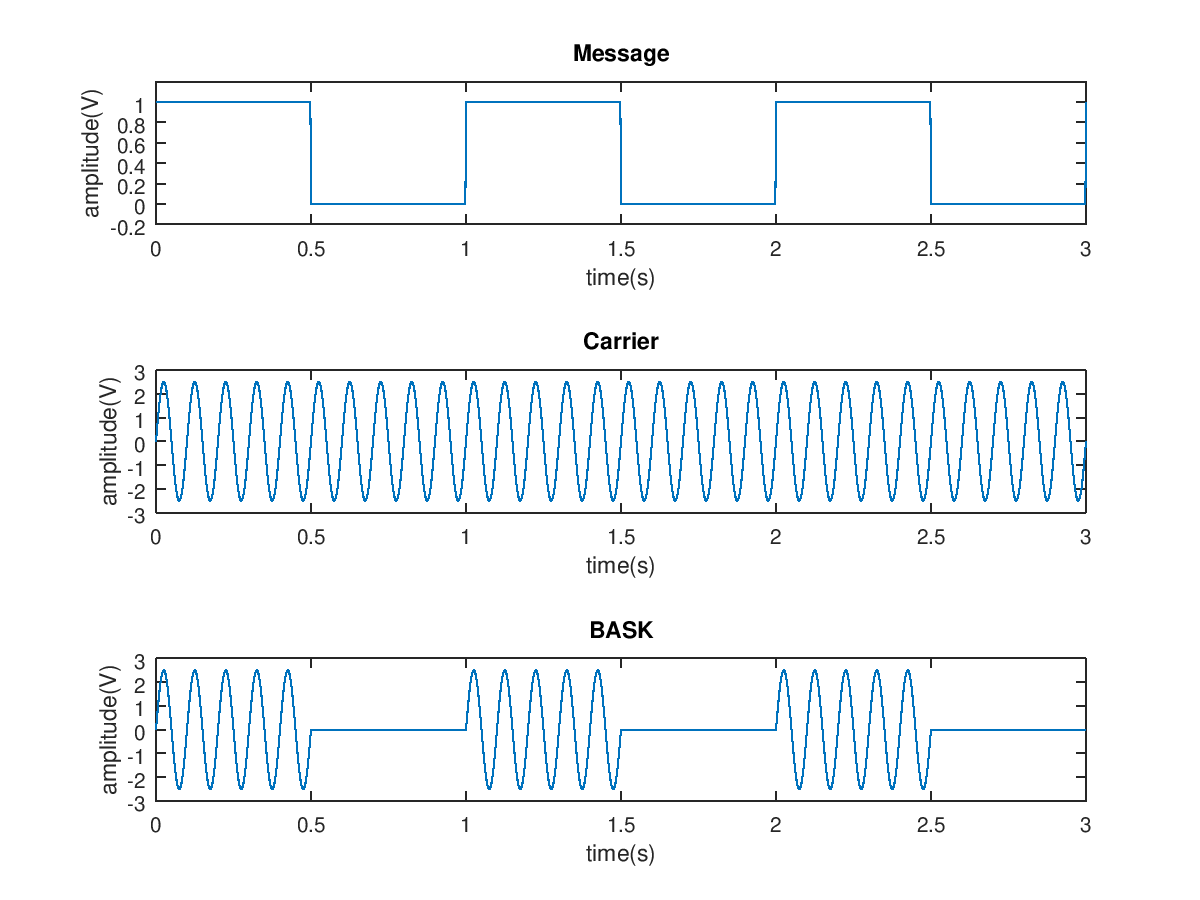
\includegraphics[width=0.8\textwidth]{baskwaves.png}
\caption{BASK sample waveforms}
\label{baskmod}
\end{figure}


\section*{Design}
\subsection*{BASK Generation}

BASK signal may be generated by simply applying the incoming binary data and sinusoidal carrier to the two inputs of an analog switch. When the binary data is applied to the control input of the switch, resulting output will be a BASK waveform. Ensure the carrier frequency is higher compared to the binary data frequency. 


\subsection*{BASK Demodulation}

Binary ASK signal can be demodulated non-coherantly using an envelop detector. This greatly simplifies the design cnsiderations required in synchronous detection. Non-coherant detection schemes  do not require a phase coherant local oscillator. 

\noindent Use 0A79 diode and $1 k\Omega $ resistor for rectification.
\noindent Use a simple RC lowpass filter to pass the low frequency binary message. Assuming the message frequecny is less than $1.5 kHz$,
 
\begin{equation}
f_H=\frac{1}{2\pi R_dC_d}
\end{equation}
\begin{equation}
1.5\ kHz=\frac{1}{2\pi R_dC_d}
\end{equation}
\noindent Select $C_d=\ 0.1 \mu F$. Then $R_d=\ 1k\Omega$.
Choose $R_d=\ 1k\Omega$ standard resistor value.\\

The resulting sequency may not be a perfect binary square wave. It can be transformed to a perfect binary sequence by using a threshold detector. The threshold level may adjusted using a $5 k\Omega$ pot.

\clearpage
\section*{Circuit Diagram}

The BASK generation using analog switching IC 4046 is shown in Figure \ref{bask-gen} and demodulation using envelop detection technique is shown in Figure \ref{bask-det}.

\begin{figure}
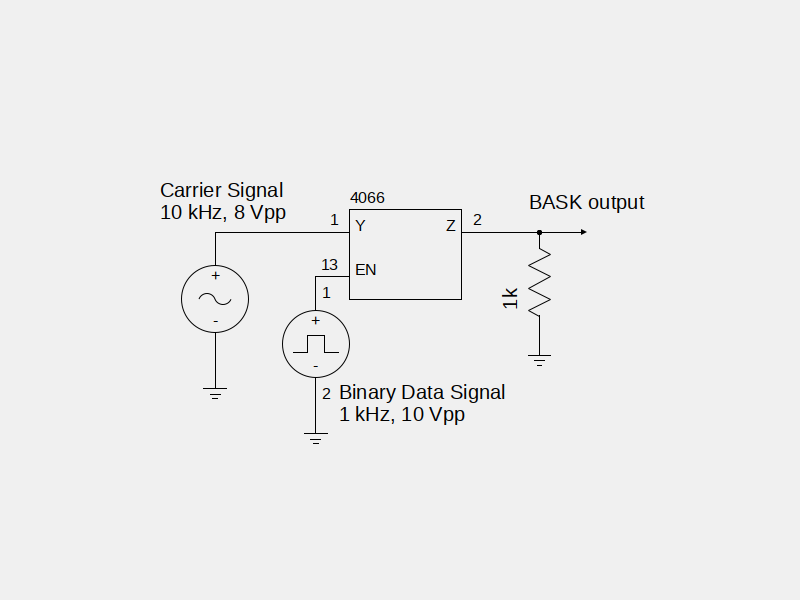
\includegraphics[width=0.8\textwidth]{bask.png}
\caption{BASK generation Circuit}
\label{bask-gen}
\end{figure}

\begin{figure}
	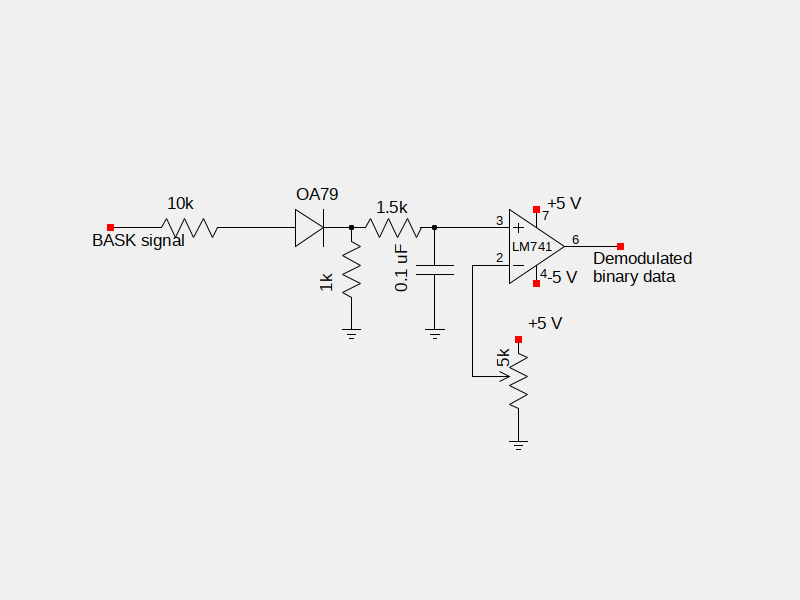
\includegraphics[width=0.8\textwidth]{bask-demod.png}
	\caption{BASK Demodulation Circuit}
	\label{bask-det}
\end{figure}


\section*{Procedure}
\begin{itemize}
\item
Connect the BASK generating circuit as shown in the circuit diagram, Figure \ref{bask-gen}.
\item
Feed the binary message data ($10 V_{pp}, 1 kHz$ square wave) and the carrier waveform  ($8 V_{pp}, 10 kHz$ sine wave) from the function generator.
\item
Observe the output on a CRO and plot the graphs of the input and output waveforms.
\item
Make the demodulating circuit as shown in the circuit diagram, Figure \ref{bask-det}.
\item
Observe the input and output waveforms from BASK demodulator.
\item 
Obtain the output of demodulator and the control input simultaneously, take the measurements and plot the waveforms.

\end{itemize}
\section*{Observation}
Plot the graphs of input and output waveforms as observed on a CRO.


\begin{figure}
	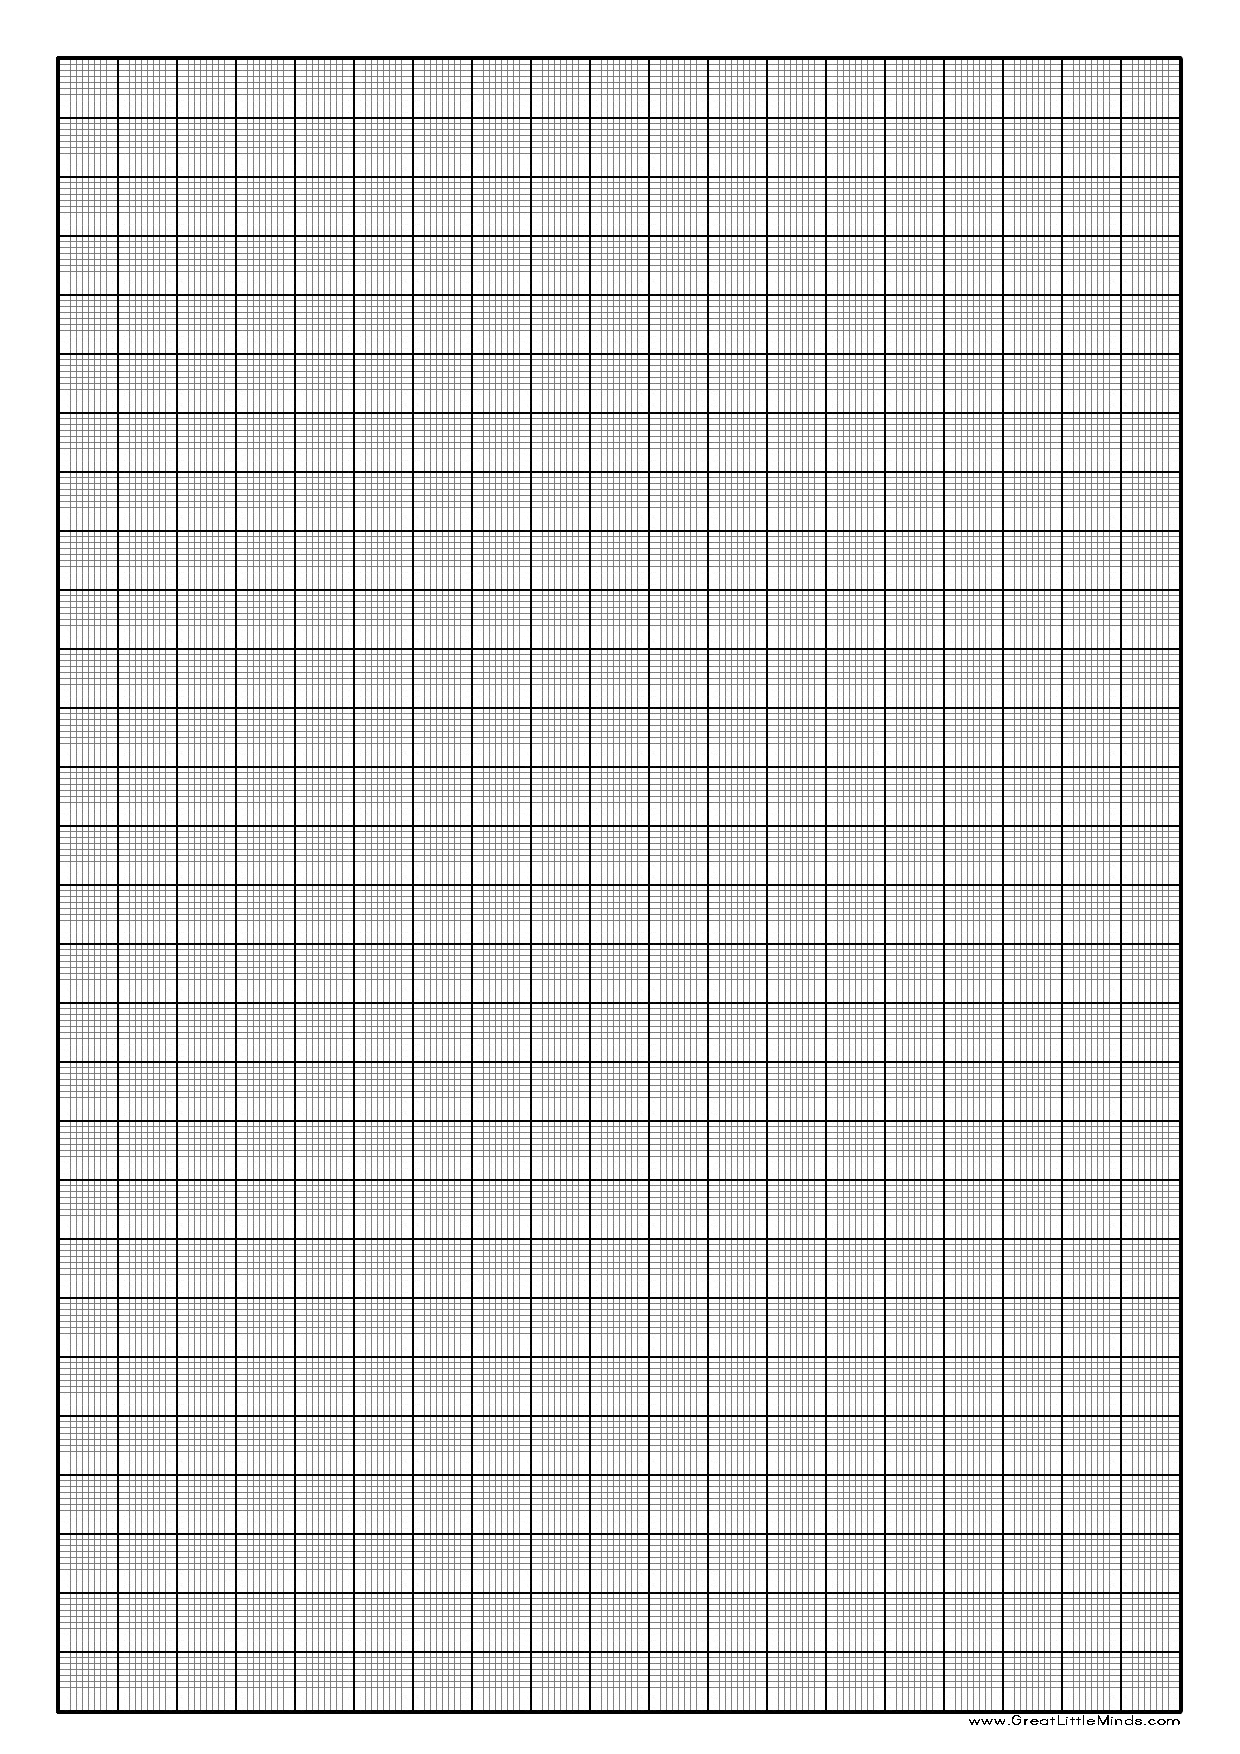
\includegraphics[width=1.1\textwidth]{graph.pdf}
\end{figure}

\section*{Result}

Implemented the BASK generation and demodulation circuits.



\begin{appendix}
\input{chapters/referencedata.tex}
\end{appendix}
\begin{thebibliography}{1}
\bibitem{ACmanual}{LABORATORY MANUAL COMMUNICATIONS LABORATORYEE 321, CALIFORNIA STATE UNIVERSITY, LOS ANGELES
Lab-Volt Systems, Inc}.
\bibitem{Bcarlson}{Communication Systems: An introduction to Signals and Noise in Electrical Communication, McGrawHill, Bruce Carlson, Paul Crilly.}

\bibitem{Tomasi}{Electronic Communication Systems- Fundamentals Through Advanced, Pearson 5ed, Wayne Tomasi}.
\bibitem{IFCAN}{\href{http://retro.co.za/archive/amateur/SM0VPO-ReusingIFCans.pdf}{REUSING TRANSISTOR IF CANS by SM0VPO}}

\bibitem{wikipll}{\href{https://en.wikipedia.org/wiki/Phase-locked_loop}{Phase Locked Loop, Wikipedia article.}}


\end{thebibliography}


\end{document}
